	\documentclass[journal,cspaper,compsoc]{IEEEtran}
\usepackage{fixltx2e}
\usepackage[nocompress]{cite}
\usepackage[pdftex]{graphicx,graphics}
\usepackage[cmex10]{amsmath}
\usepackage{amssymb,amsthm}
\usepackage{url}
\usepackage{float}
\usepackage[inline]{enumitem}
\usepackage{subfig}	
\usepackage{array}
%\usepackage{booktabs}
\usepackage{algorithmic}
\usepackage[linesnumbered, boxed, commentsnumbered, ruled, vlined]{algorithm2e}
\usepackage{makecell}
\usepackage{multirow}
\usepackage{booktabs}
\usepackage{color}
\usepackage{amsfonts}
\usepackage[normalem]{ulem}



\begin{document}

\newtheorem{definition}{Definition}[section]
\newtheorem{ex}{Example}[section]
\newtheorem{lemma}{Lemma}[section]
\newtheorem{theorem}{Theorem}[section]
%\newtheorem{proof}{Proof}[section]

\title{Risk-Aware Sensitive Property-Driven
Resource Management in Cloud Datacenters}

\author{% <-this % stops a space
Muhamad Felemban, \textit{Member, IEEE}, Abdulrahman Almutairi, and Arif Ghafoor, \textit{Fellow, IEEE}
\IEEEcompsocitemizethanks{\IEEEcompsocthanksitem M. Felemban is with the Computer Engineering Department, the Information and Computer Science Department, and the Interdisciplinary Research Center for Intelligent Secure Systems at KFUPM. 
\IEEEcompsocthanksitem A. Ghafoor is with the School of Electrical and Computer Engineering and Purdue's Center for Education and Research in Information Assurance and Security~(CERIAS), Purdue University, West Lafayette,IN, \IEEEcompsocthanksitem A. Almutairi is with the Computer Engineering Department at the College of Computer and Information Science  in King Saud University, Riyadh, Saudi Arabia }}


\IEEEcompsoctitleabstractindextext{
\begin{abstract}
\begin{abstract}  
Test time scaling is currently one of the most active research areas that shows promise after training time scaling has reached its limits.
Deep-thinking (DT) models are a class of recurrent models that can perform easy-to-hard generalization by assigning more compute to harder test samples.
However, due to their inability to determine the complexity of a test sample, DT models have to use a large amount of computation for both easy and hard test samples.
Excessive test time computation is wasteful and can cause the ``overthinking'' problem where more test time computation leads to worse results.
In this paper, we introduce a test time training method for determining the optimal amount of computation needed for each sample during test time.
We also propose Conv-LiGRU, a novel recurrent architecture for efficient and robust visual reasoning. 
Extensive experiments demonstrate that Conv-LiGRU is more stable than DT, effectively mitigates the ``overthinking'' phenomenon, and achieves superior accuracy.
\end{abstract}  
\end{abstract}
\begin{IEEEkeywords}
Cloud services, access control, risk assessment, vulnerability
\end{IEEEkeywords}}

\maketitle


\section{Introduction}\label{sec:introduction}
\section{Introduction}
\label{sec:introduction}
The business processes of organizations are experiencing ever-increasing complexity due to the large amount of data, high number of users, and high-tech devices involved \cite{martin2021pmopportunitieschallenges, beerepoot2023biggestbpmproblems}. This complexity may cause business processes to deviate from normal control flow due to unforeseen and disruptive anomalies \cite{adams2023proceddsriftdetection}. These control-flow anomalies manifest as unknown, skipped, and wrongly-ordered activities in the traces of event logs monitored from the execution of business processes \cite{ko2023adsystematicreview}. For the sake of clarity, let us consider an illustrative example of such anomalies. Figure \ref{FP_ANOMALIES} shows a so-called event log footprint, which captures the control flow relations of four activities of a hypothetical event log. In particular, this footprint captures the control-flow relations between activities \texttt{a}, \texttt{b}, \texttt{c} and \texttt{d}. These are the causal ($\rightarrow$) relation, concurrent ($\parallel$) relation, and other ($\#$) relations such as exclusivity or non-local dependency \cite{aalst2022pmhandbook}. In addition, on the right are six traces, of which five exhibit skipped, wrongly-ordered and unknown control-flow anomalies. For example, $\langle$\texttt{a b d}$\rangle$ has a skipped activity, which is \texttt{c}. Because of this skipped activity, the control-flow relation \texttt{b}$\,\#\,$\texttt{d} is violated, since \texttt{d} directly follows \texttt{b} in the anomalous trace.
\begin{figure}[!t]
\centering
\includegraphics[width=0.9\columnwidth]{images/FP_ANOMALIES.png}
\caption{An example event log footprint with six traces, of which five exhibit control-flow anomalies.}
\label{FP_ANOMALIES}
\end{figure}

\subsection{Control-flow anomaly detection}
Control-flow anomaly detection techniques aim to characterize the normal control flow from event logs and verify whether these deviations occur in new event logs \cite{ko2023adsystematicreview}. To develop control-flow anomaly detection techniques, \revision{process mining} has seen widespread adoption owing to process discovery and \revision{conformance checking}. On the one hand, process discovery is a set of algorithms that encode control-flow relations as a set of model elements and constraints according to a given modeling formalism \cite{aalst2022pmhandbook}; hereafter, we refer to the Petri net, a widespread modeling formalism. On the other hand, \revision{conformance checking} is an explainable set of algorithms that allows linking any deviations with the reference Petri net and providing the fitness measure, namely a measure of how much the Petri net fits the new event log \cite{aalst2022pmhandbook}. Many control-flow anomaly detection techniques based on \revision{conformance checking} (hereafter, \revision{conformance checking}-based techniques) use the fitness measure to determine whether an event log is anomalous \cite{bezerra2009pmad, bezerra2013adlogspais, myers2018icsadpm, pecchia2020applicationfailuresanalysispm}. 

The scientific literature also includes many \revision{conformance checking}-independent techniques for control-flow anomaly detection that combine specific types of trace encodings with machine/deep learning \cite{ko2023adsystematicreview, tavares2023pmtraceencoding}. Whereas these techniques are very effective, their explainability is challenging due to both the type of trace encoding employed and the machine/deep learning model used \cite{rawal2022trustworthyaiadvances,li2023explainablead}. Hence, in the following, we focus on the shortcomings of \revision{conformance checking}-based techniques to investigate whether it is possible to support the development of competitive control-flow anomaly detection techniques while maintaining the explainable nature of \revision{conformance checking}.
\begin{figure}[!t]
\centering
\includegraphics[width=\columnwidth]{images/HIGH_LEVEL_VIEW.png}
\caption{A high-level view of the proposed framework for combining \revision{process mining}-based feature extraction with dimensionality reduction for control-flow anomaly detection.}
\label{HIGH_LEVEL_VIEW}
\end{figure}

\subsection{Shortcomings of \revision{conformance checking}-based techniques}
Unfortunately, the detection effectiveness of \revision{conformance checking}-based techniques is affected by noisy data and low-quality Petri nets, which may be due to human errors in the modeling process or representational bias of process discovery algorithms \cite{bezerra2013adlogspais, pecchia2020applicationfailuresanalysispm, aalst2016pm}. Specifically, on the one hand, noisy data may introduce infrequent and deceptive control-flow relations that may result in inconsistent fitness measures, whereas, on the other hand, checking event logs against a low-quality Petri net could lead to an unreliable distribution of fitness measures. Nonetheless, such Petri nets can still be used as references to obtain insightful information for \revision{process mining}-based feature extraction, supporting the development of competitive and explainable \revision{conformance checking}-based techniques for control-flow anomaly detection despite the problems above. For example, a few works outline that token-based \revision{conformance checking} can be used for \revision{process mining}-based feature extraction to build tabular data and develop effective \revision{conformance checking}-based techniques for control-flow anomaly detection \cite{singh2022lapmsh, debenedictis2023dtadiiot}. However, to the best of our knowledge, the scientific literature lacks a structured proposal for \revision{process mining}-based feature extraction using the state-of-the-art \revision{conformance checking} variant, namely alignment-based \revision{conformance checking}.

\subsection{Contributions}
We propose a novel \revision{process mining}-based feature extraction approach with alignment-based \revision{conformance checking}. This variant aligns the deviating control flow with a reference Petri net; the resulting alignment can be inspected to extract additional statistics such as the number of times a given activity caused mismatches \cite{aalst2022pmhandbook}. We integrate this approach into a flexible and explainable framework for developing techniques for control-flow anomaly detection. The framework combines \revision{process mining}-based feature extraction and dimensionality reduction to handle high-dimensional feature sets, achieve detection effectiveness, and support explainability. Notably, in addition to our proposed \revision{process mining}-based feature extraction approach, the framework allows employing other approaches, enabling a fair comparison of multiple \revision{conformance checking}-based and \revision{conformance checking}-independent techniques for control-flow anomaly detection. Figure \ref{HIGH_LEVEL_VIEW} shows a high-level view of the framework. Business processes are monitored, and event logs obtained from the database of information systems. Subsequently, \revision{process mining}-based feature extraction is applied to these event logs and tabular data input to dimensionality reduction to identify control-flow anomalies. We apply several \revision{conformance checking}-based and \revision{conformance checking}-independent framework techniques to publicly available datasets, simulated data of a case study from railways, and real-world data of a case study from healthcare. We show that the framework techniques implementing our approach outperform the baseline \revision{conformance checking}-based techniques while maintaining the explainable nature of \revision{conformance checking}.

In summary, the contributions of this paper are as follows.
\begin{itemize}
    \item{
        A novel \revision{process mining}-based feature extraction approach to support the development of competitive and explainable \revision{conformance checking}-based techniques for control-flow anomaly detection.
    }
    \item{
        A flexible and explainable framework for developing techniques for control-flow anomaly detection using \revision{process mining}-based feature extraction and dimensionality reduction.
    }
    \item{
        Application to synthetic and real-world datasets of several \revision{conformance checking}-based and \revision{conformance checking}-independent framework techniques, evaluating their detection effectiveness and explainability.
    }
\end{itemize}

The rest of the paper is organized as follows.
\begin{itemize}
    \item Section \ref{sec:related_work} reviews the existing techniques for control-flow anomaly detection, categorizing them into \revision{conformance checking}-based and \revision{conformance checking}-independent techniques.
    \item Section \ref{sec:abccfe} provides the preliminaries of \revision{process mining} to establish the notation used throughout the paper, and delves into the details of the proposed \revision{process mining}-based feature extraction approach with alignment-based \revision{conformance checking}.
    \item Section \ref{sec:framework} describes the framework for developing \revision{conformance checking}-based and \revision{conformance checking}-independent techniques for control-flow anomaly detection that combine \revision{process mining}-based feature extraction and dimensionality reduction.
    \item Section \ref{sec:evaluation} presents the experiments conducted with multiple framework and baseline techniques using data from publicly available datasets and case studies.
    \item Section \ref{sec:conclusions} draws the conclusions and presents future work.
\end{itemize}

\section{Cloud Vulnerability and Authorization Policy for Datacenters}\label{sec:profile}
\section{Background}\label{sec:backgrnd}

\subsection{Cold Start Latency and Mitigation Techniques}

Traditional FaaS platforms mitigate cold starts through snapshotting, lightweight virtualization, and warm-state management. Snapshot-based methods like \textbf{REAP} and \textbf{Catalyzer} reduce initialization time by preloading or restoring container states but require significant memory and I/O resources, limiting scalability~\cite{dong_catalyzer_2020, ustiugov_benchmarking_2021}. Lightweight virtualization solutions, such as \textbf{Firecracker} microVMs, achieve fast startup times with strong isolation but depend on robust infrastructure, making them less adaptable to fluctuating workloads~\cite{agache_firecracker_2020}. Warm-state management techniques like \textbf{Faa\$T}~\cite{romero_faa_2021} and \textbf{Kraken}~\cite{vivek_kraken_2021} keep frequently invoked containers ready, balancing readiness and cost efficiency under predictable workloads but incurring overhead when demand is erratic~\cite{romero_faa_2021, vivek_kraken_2021}. While these methods perform well in resource-rich cloud environments, their resource intensity challenges applicability in edge settings.

\subsubsection{Edge FaaS Perspective}

In edge environments, cold start mitigation emphasizes lightweight designs, resource sharing, and hybrid task distribution. Lightweight execution environments like unikernels~\cite{edward_sock_2018} and \textbf{Firecracker}~\cite{agache_firecracker_2020}, as used by \textbf{TinyFaaS}~\cite{pfandzelter_tinyfaas_2020}, minimize resource usage and initialization delays but require careful orchestration to avoid resource contention. Function co-location, demonstrated by \textbf{Photons}~\cite{v_dukic_photons_2020}, reduces redundant initializations by sharing runtime resources among related functions, though this complicates isolation in multi-tenant setups~\cite{v_dukic_photons_2020}. Hybrid offloading frameworks like \textbf{GeoFaaS}~\cite{malekabbasi_geofaas_2024} balance edge-cloud workloads by offloading latency-tolerant tasks to the cloud and reserving edge resources for real-time operations, requiring reliable connectivity and efficient task management. These edge-specific strategies address cold starts effectively but introduce challenges in scalability and orchestration.

\subsection{Predictive Scaling and Caching Techniques}

Efficient resource allocation is vital for maintaining low latency and high availability in serverless platforms. Predictive scaling and caching techniques dynamically provision resources and reduce cold start latency by leveraging workload prediction and state retention.
Traditional FaaS platforms use predictive scaling and caching to optimize resources, employing techniques (OFC, FaasCache) to reduce cold starts. However, these methods rely on centralized orchestration and workload predictability, limiting their effectiveness in dynamic, resource-constrained edge environments.



\subsubsection{Edge FaaS Perspective}

Edge FaaS platforms adapt predictive scaling and caching techniques to constrain resources and heterogeneous environments. \textbf{EDGE-Cache}~\cite{kim_delay-aware_2022} uses traffic profiling to selectively retain high-priority functions, reducing memory overhead while maintaining readiness for frequent requests. Hybrid frameworks like \textbf{GeoFaaS}~\cite{malekabbasi_geofaas_2024} implement distributed caching to balance resources between edge and cloud nodes, enabling low-latency processing for critical tasks while offloading less critical workloads. Machine learning methods, such as clustering-based workload predictors~\cite{gao_machine_2020} and GRU-based models~\cite{guo_applying_2018}, enhance resource provisioning in edge systems by efficiently forecasting workload spikes. These innovations effectively address cold start challenges in edge environments, though their dependency on accurate predictions and robust orchestration poses scalability challenges.

\subsection{Decentralized Orchestration, Function Placement, and Scheduling}

Efficient orchestration in serverless platforms involves workload distribution, resource optimization, and performance assurance. While traditional FaaS platforms rely on centralized control, edge environments require decentralized and adaptive strategies to address unique challenges such as resource constraints and heterogeneous hardware.



\subsubsection{Edge FaaS Perspective}

Edge FaaS platforms adopt decentralized and adaptive orchestration frameworks to meet the demands of resource-constrained environments. Systems like \textbf{Wukong} distribute scheduling across edge nodes, enhancing data locality and scalability while reducing network latency. Lightweight frameworks such as \textbf{OpenWhisk Lite}~\cite{kravchenko_kpavelopenwhisk-light_2024} optimize resource allocation by decentralizing scheduling policies, minimizing cold starts and latency in edge setups~\cite{benjamin_wukong_2020}. Hybrid solutions like \textbf{OpenFaaS}~\cite{noauthor_openfaasfaas_2024} and \textbf{EdgeMatrix}~\cite{shen_edgematrix_2023} combine edge-cloud orchestration to balance resource utilization, retaining latency-sensitive functions at the edge while offloading non-critical workloads to the cloud. While these approaches improve flexibility, they face challenges in maintaining coordination and ensuring consistent performance across distributed nodes.



\section{Problem Definition and Formulation}\label{sec:assignment}
\section{Problem Formulation} \label{sec:probdef}

This section formally defines the problem of restoring a given pruned network with only using its original pretrained CNN in a way free of data and fine-tuning.



% Unlike many existing works utilize data for identifying unimportant filters as well as fine-tuning to this end, we cannot evaluate the filter importance by data-dependent values like activation maps (\textit{a.k.a.} channels) as our focus in this paper is not to use any training data. Thus, in our problem setting, we can only exploit the values of filters in the original network, and thereby have to make some changes in the remaining filters of the pruned network so that the network can return the output not too much different from the original one.

% No matter how much we carefully select unimportant filters to be pruned, some kinds of retraining process appears inevitable as done by the most existing works to this end. However, since our focus in this paper is not to use any training data, we cannot evaluate the importance of filters by data-dependent values like activation maps (\textit{a.k.a.} channels). 

% To this end, they not only use a careful criterion (\textit{e.g.}, L1-norm), but also fine-tune the network using the original data.
% Most of filter pruning methods try to select filters to be pruned prudently so that pruned network's output be similar to the original network's. To this end, they prune the unimportant filters and then fine-tune the pruned network with using the train data. 

% How can we restore the the pruned networks without any data? In other words, it implies that we cannot use any data-driven values(i.e., activation maps) and we can only exploit the values of original filters. In that case, the only thing we can do maybe changing the weights of remained filters appropriately not to amplify the difference between pruned and unpruned network's outputs through the information of original filters.

\begin{figure*}[t]
	\centering
    \subfigure[\label{fig:matrix:a}Pruning matrix]{\hspace{6mm}\includegraphics[width=0.35\columnwidth]{./figure/LBYL_figure_2_1.pdf}\hspace{6mm}} 
    \subfigure[\label{fig:matrix:b}Delivery matrix for LBYL]{\hspace{6mm}\includegraphics[width=0.35\columnwidth]{./figure/LBYL_figure_2_2.pdf}\hspace{6mm}}
    \subfigure[\label{fig:matrix:c}Delivery matrix for one-to-one]{\hspace{9mm}\includegraphics[width=0.35\columnwidth]{./figure/LBYL_figure_2_3.pdf}\hspace{9mm}} 
    \caption{Comparison between pruning matrix and delivery matrix, where the $4$-th and $6$-th filters are being pruned among $6$ original filters}
	\label{fig:matrix}
	\vspace{-2mm}
\end{figure*}



\subsection{Filter Pruning in a CNN}
Consider a given CNN to be pruned with $L$ layers, where each $\ell$-th layer starts with a convolution operation on its input channels, which are the output of the previous $(\ell-1)$-th layer $\mathbf{A}^{(\ell-1)}$, with the group of convolution filters $\mathbf{W}^{{(\ell)}}$ and thereby obtain the set of \textit{feature maps} $\mathbf{Z}^{(\ell)}$ as follows:
\begin{equation}
\boldsymbol{\mathbf{Z}}^{(\ell)} = {\mathbf{A}^{(\ell-1)} \circledast {\mathbf{W}}^{(\ell)}},
\nonumber
\end{equation}
where $\circledast$ represents the convolution operation. Then, this convolution process is normally followed by a batch normalization (BN) process and an activation function such as ReLU, and the $\ell$-th layer finally outputs an \textit{activation map} $\mathbf{A}^{(\ell)}$ to be sent to the $(\ell+1)$-th layer through this sequence of procedures as:
\begin{equation}
\mathbf{A}^{(\ell)} = \F(\N(\mathbf{Z}^{(\ell)})),
\nonumber
\end{equation}
where $\F(\cdot)$ is an activation function and $\N(\cdot)$ is a BN procedure.

Note that all of $\mathbf{W}^{(\ell)}$, $\mathbf{Z}^{(\ell)}$, and $\mathbf{A}^{(\ell)}$ are tensors such that: $\mathbf{W}^{(\ell)} \in \mathbb{R}^{m \times n \times k \times k}$ and $\mathbf{Z}^{(\ell)},\mathbf{A}^{(\ell)} \in \mathbb{R}^{m \times w \times h}$, where (1) $m$ is the number of filters, which also equals the number of output activation maps, (2) $n$ is the number of input activation maps resulting from the $(\ell-1)$-th layer, (3) $k \times k$ is the size of each filter, and (4) $w \times h$ is the size of each output channel for the $\ell$-th layer.

\smalltitle{Filter pruning as n-mode product}
When filter pruning is performed at the $\ell$-th layer, all three tensors above are consequently modified to their \textit{damaged} versions, namely $\mathbf{\Tilde{W}}^{(\ell)}$, $\mathbf{\Tilde{Z}}^{(\ell)}$, and $\mathbf{\Tilde{A}}^{(\ell)}$, respectively, in a way that: $\mathbf{\Tilde{W}}^{(\ell)} \in \mathbb{R}^{t \times n \times k \times k}$ and $\mathbf{\Tilde{Z}}^{(\ell)},\mathbf{\Tilde{A}}^{(\ell)} \in \mathbb{R}^{t \times w \times h}$, where $t$ is the number of remaining filters after pruning and therefore $t < m$. Mathematically, the tensor of remaining filters, \textit{i.e.}, $\mathbf{\Tilde{W}}^{(\ell)}$, is obtained by the \textit{$1$-mode product} \cite{DBLP:journals/siamrev/KoldaB09} of the tensor of the original filters $\mathbf{W}^{(\ell)}$ with a \textit{pruning matrix} $\boldsymbol{\S} \in \mathbb{R}^{m \times t}$ (see Figure \ref{fig:matrix:a})
as follows:
\begin{eqnarray}\begin{split}\label{eq:pruning}
\mathbf{\Tilde{W}}^{(\ell)} = {\mathbf{W}}^{(\ell)} \times_{1} {\boldsymbol{\S}}^{T},\text{where }\boldsymbol{\S}_{i,k} = 
  \begin{cases} 
   1~ \text{if } i = i'_k \\
   0~ \text{otherwise}
  \end{cases} \\
  \text{s.t. } i, i'_k \in [1, m] 
  \text{ and } k \in [1, t].
  \end{split}
\end{eqnarray}
  
By Eq. (\ref{eq:pruning}), each $i'_k$-th filter is not pruned and the other $(m-t)$ filters are completely removed from $\mathbf{W}^{(\ell)}$ to be $\mathbf{\Tilde{W}}^{(\ell)}$.

This reduction at the $\ell$-th layer causes another reduction for each filter of the $(\ell+1)$-th layer so that $\mathbf{W}^{(\ell+1)}$ is now modified to $\mathbf{\Tilde{W}}^{(\ell+1)} \in \mathbb{R}^{m' \times t \times k' \times k'}$, where $m'$ is the number of filters of size $k' \times k'$ in the $(\ell+1)$-th layer. Due to this series of information losses, the resulting feature map (\textit{i.e.}, $\mathbf{Z}^{(\ell+1)}$) would severely be damaged to be $\mathbf{\Tilde{Z}}^{(\ell+1)}$ as shown below:
\begin{equation}
{\mathbf{\Tilde{Z}}}^{{(\ell+1)}} = \mathbf{\Tilde{A}}^{(\ell)} \circledast {\mathbf{\Tilde{W}}}^{(\ell+1)}~~~\not\approx~~~\mathbf{Z}^{(\ell+1)}
\label{eq:eq}\nonumber
\end{equation}
The shape of $\mathbf{\Tilde{Z}}^{(\ell+1)}$ remains the same unless we also prune filters for the $(\ell+1)$-th layer. If we do so as well, the loss of information will be accumulated and further propagated to the next layers. Note that $\mathbf{\Tilde{W}}^{(\ell+1)}$ can also be represented by the \textit{$2$-mode product} \cite{DBLP:journals/siamrev/KoldaB09} of $\mathbf{W}^{(\ell+1)}$ with the transpose of the same matrix $\boldsymbol{\S}$ as:
\begin{equation} \label{eq:pruning2}
\mathbf{\Tilde{W}}^{(\ell+1)} = {\mathbf{W}}^{(\ell+1)} \times_{2} {\boldsymbol{\S}^T}
\end{equation}




\subsection{Problem of Restoring a Pruned Network without Data and Fine-Tuning}
As mentioned earlier, our goal is to restore a pruned and thus damaged CNN without using any data and re-training process, which implies the following two facts. First, we have to use a pruning criterion exploiting only the values of filters themselves such as L1-norm. In this sense, this paper does not focus on proposing a sophisticated pruning criterion but intends to recover a network somehow pruned by such a simple criterion. Secondly, since we cannot make appropriate changes in the remaining filters by fine-tuning, we should make the best use of the original network and identify how the information carried by a pruned filter can be delivered to the remaining filters.

% For brevity, we formulate our problem here with respect to a specific layer, say $\ell$, and then it can trivially be generalized for the entire network. 
\smalltitle{Delivery matrix}
In order to represent the information to be delivered to the preserved filters, let us first think of what the pruning matrix $\boldsymbol{\S}$ means. As defined in Eq. (\ref{eq:pruning}) and shown in Figure \ref{fig:matrix:a}, each row is either a zero vector (for filters being pruned) or a one-hot vector (for remaining filters), which is intended only to remove filters without delivering any information. Intuitively, we can transform this pruning matrix into a \textit{delivery matrix} that carries information for filters being pruned by replacing some meaningful values with some of the zero values therein. Once we find such an \textit{ideal} $\boldsymbol{\S^*}$, we can plug it into $\boldsymbol{\S}$ of Eq. (\ref{eq:pruning2}) to deliver missing information propagated from the $\ell$-th layer to the filters at the $(\ell+1)$-th layer, which will hopefully generate an approximation $\mathbf{\hat{Z}}^{(\ell+1)}$ close to the original feature map as follows:
\begin{equation} \label{eq:fmap_approx}
{\mathbf{\hat{Z}}}^{{(\ell+1)}} = {\mathbf{\Tilde{A}}^{(\ell)} \circledast ({\mathbf{W}}^{(\ell+1)} \times_{2} {\boldsymbol{\S^*}^T})}
~~~\approx~~~\mathbf{Z}^{(\ell+1)}
\end{equation}
Thus, using the delivery matrix $\boldsymbol{\mathcal{S^*}}$, the information loss caused by pruning at each layer is recovered at the feature map of the next layer.

\smalltitle{Problem statement}
Given a pretrained CNN, our problem aims to find the best delivery matrix $\boldsymbol{\mathcal{S^*}}$ for each layer without any data and training process such that the following \textit{reconstruction error} is minimized:
\begin{equation}
\sum\limits_{i = 1}^{m'}\|{{\mathbf{Z}}_{i}^{{(\ell+1)}}-{\hat{\mathbf{Z}}}_{i}^{{(\ell+1)}}}\|_1,
\label{eq:goal}
\end{equation}
where ${\mathbf{Z}}_i^{{(\ell+1)}}$ and ${\hat{\mathbf{Z}}}_i^{{(\ell+1)}}$ indicate the $i$-th original feature map and its corresponding approximation, respectively, out of $m'$ filters in the $(\ell+1)$-th layer. Note that what is challenging here is that we cannot obtain the activation maps in $\mathbf{A}^{(\ell)}$ and $\mathbf{\Tilde{A}}^{(\ell)}$ without data as they are data-dependent values.

% = \sum\limits_{i = 1}^{m'}\|{{\mathbf{Z}}_{i}^{{(\ell+1)}}-{\mathbf{\Tilde{A}}^{(\ell)} \circledast ({\mathbf{W}}^{(\ell+1)} \times_{2} {\boldsymbol{\mathcal{S^*}^T}})}}\|_{1}


% Our goal is finding the approximation matrix $\boldsymbol{\mathcal{S}}$ to minimize the reconstruction error between the pruned model and the original model without any data, and effectively deliver missing information for pruned filters using this approximation matrix


% $\testit{s}$,which can be represented as below.

% \begin{equation}
% \boldsymbol{\mathcal{S}} =  \underset{{\boldsymbol{\mathcal{S}}}}{\mathrm{argmin}} \sum\limits_{{i} = 1}^{m_{\ell+1}} \|{{\mathbf{Z}}_{i,:,:}^{{(\ell+1)}}-{\hat{\mathbf{Z}}}_{i,:,:}^{{(\ell+1)}}}\|_{1} 
% \label{eq:eq1}
% \end{equation}



% Let us first recall that the ultimate goal of network pruning is to make the output of a pruned network as close as possible to that of its original network. Unlike many existing pruning methods, our focus is not to use any training data at all for the entire pruning and recovery process, and this implies the following two facts. First, we cannot evaluate the filter importance by data-dependent values like activation values or gradients, but have to use a pruning criterion exploiting only the values of filters themselves such as L1-norm. Furthermore, instead of fine-tuning with data, the only thing we can do for the pruned network is to make appropriate changes in the remaining filters by identifying some relationships between pruned filters and the other preserved ones without any support from data. Based on this intuition, this section mathematically and generally defines the problem of restoring a pruned neural network in a manner free of data and fine-tuning.


% Thus, we make approximation matrix $\testit{s}$ $\in$ $\mathbb{R}^{m_{\ell} \times t_{\ell}}$ with relationship between the pruned filter and preserved filters in $\ell$-th layer and then apply it to the original filters in $(\ell+1)$-th layer to compensate for pruned feature maps $\boldsymbol{\hat{\mathbf{Z}}}^{{(\ell+1)}}$ as shown below.
% (\textit{i.e.}, Let $\hat{\mathbf{W}}^{(\ell+1)}$ be ${\mathbf{W}}^{(\ell+1)}$ $\times_2$ ${{\textit{s}}} $, where $\times_2$ is 2-mode matrix product) 

% \begin{equation}
% \mathbf{Z}^{(\ell+1)} = {\mathbf{A}}^{(\ell)} \circledast {\mathbf{W}}^{(\ell+1)}
% \approx {\hat{\mathbf{A}}^{(\ell)} \circledast ({\mathbf{W}}^{(\ell+1)} \times_{2} {{s}}) = {\hat{\mathbf{Z}}}^{{(\ell+1)}}}
% \label{eq:eq}\nonumber
% \end{equation}




% For a Convolutional Neural Network (CNN) with $L$ layers, we denote $\mathcal{A}{^{(\ell-1)}}$ $\in$ $\mathbb{R}^{n_{\ell -1 } \times h_{\ell -1} \times w_{\ell -1}}$ is activation maps at $\ell-1$-th layer, where $n_{\ell -1}$, $h_{\ell -1}$ and $w_{\ell -1}$ are the number of channels, height and width in activation maps, respectively. and we denote $\mathbf{W}^{{(\ell )}}$ $\in$  $\mathbb{R}^{m_{\ell} \times n_{\ell -1}\times k \times k}$ is covolution filters in $\ell$-th layer,where $m_{\ell}$, $n_{\ell-1}$ and $k$ are the number of filters, number of channels and kernel size, respectively. Trough the convolution operation using activation map $\mathcal{A}{^{(\ell-1)}}$ and convolution filter $\mathbf{W}^{{(\ell)}}$ in $\ell$-th layer, the feature maps $\boldsymbol{\mathbf{Z}}^{{(\ell)}}$ $\in$ $\mathbb{R}^{m_{\ell} \times h_{\ell+1} \times w_{\ell+1}}$ is computed as shown as below.


% \begin{equation}
% \boldsymbol{\mathbf{Z}}^{(\ell)} = {\mathcal{A}^{(\ell-1)} \circledast {\mathbf{W}}^{(\ell)}}
% \label{eq:eq1}\nonumber
% \end{equation}
% where $\circledast$ is convolution operation.

% and the feature maps passed through the BN and ReLU layer are activation maps $\mathcal{A}{^{(\ell)}}$ $\in$ $\mathbb{R}^{m_{{\ell}} \times h_{\ell+1} \times w_{\ell+1}} $ in $\ell$-th layer as shown as below.

% \begin{equation}
% \mathcal{A}^{(\ell)} = \mathcal{F}(\mathbf{Z}^{(\ell)} \circledast {\mathbf{W}}^{(\ell)})
% \label{eq:eq2}\nonumber
% \end{equation}
% where $\mathcal{F}$ is the function that implement batch normalization and non-linear activation(\textit{e.g.}, ReLU).

% \smalltitle{Filter Pruning}
% If the filter pruning is performed in $\ell$-th layer, the shape of original filters $\mathbf{W}^{{(\ell)}}$ $\in$ $\mathbb{R}^{m_{\ell} \times n_{\ell-1}\times k \times k}$ is modified to ${\hat {\mathbf{W}}^{(\ell)}}$ $\in$ $\mathbb{R}^{t_{\ell} \times n_{\ell-1}\times k \times k}$, where $t_{\ell}$ $<$ $m_{\ell}$ by pruning criterion. Therefore, the pruned activation maps ${\hat {\mathcal{A}}}{^{({\ell+1})}}$ $\in$ $\mathbb{R}^{t_{{\ell}} \times h_{{\ell+2}} \times w_{{\ell+2}}}$ in (${\ell+1}$)-th layer is computed as below.

% \begin{equation}
% \mathbf{\hat{A}}^{(l+1)} = \mathcal{F}({\mathbf{A}^{(\ell)} \circledast {\mathbf{\hat{W}}}^{(\ell+1)}})
% \label{eq:eq3}\nonumber
% \end{equation}

% Moreover, corresponding channels of each filters in ($\ell +1$)-th layer are sequentially removed. As a result, shape of original filters $\mathbf{W}^{{(\ell+1)}}$ $\in$ $\mathbb{R}^{m_{\ell+1} \times m_{\ell}\times k \times k}$ in ($\ell+1$)-th layer is changed to  ${\hat {\mathbf{W}}^{(\ell+1)}}$ $\in$ $\mathbb{R}^{m_{\ell+1} \times t_{\ell}\times k \times k}$. Although feature maps ${\hat{\mathbf{Z}}}^{{(\ell+1)}}$ $\in$ $\mathbb{R}^{m_{\ell+1} \times h_{\ell+2} \times w_{\ell+2}}$ in ($\ell+1$)-th layer after pruning have same shape with original feature maps ${\mathbf{Z}}^{{(\ell+1)}}$ $\in$ $\mathbb{R}^{m_{\ell+1} \times h_{\ell+2} \times w_{\ell+2}}$, the pruned feature maps $\boldsymbol{\hat{\mathbf{Z}}}^{{(\ell+1)}}$ are damaged.

\section{Proposed Heuristics for RSPAP}\label{sec:heuristics}
In this section, we propose two heuristics for solving RKAP which can be used by the resource assignment component in VRM in Figure \ref{fig:arch}. The first heuristic follows a top-down clustering based approach. In each step, the cluster of roles is divided based on the risk associated with the disclosure of the sensitive property. The second heuristic is a neighbor-based heuristic, which uses a pairwise property disclosure measure for role scheduling. This measure is computed based on the inference function $f$. Each role is assigned to the best available virtual resource with respect to the probability of leakage.

\subsection{Top-Down Heuristic (TDH)}
In  this heuristic, a top down clustering approach is used. Initially, all the roles are assumed to be in one cluster. We begin with division of this root cluster and split it into two clusters such that total measure of property disclosure $g_i^A $ of both clusters is minimum. The resulting clusters are sorted based on their total $g_i^A$. TDH splits a cluster with the largest total $g_i^A$ further by moving roles with high value of $g_i^A$ from current cluster to the new cluster such that the total $g_i^A$ of both clusters is minimum. TDH repeats the cluster  splitting  step until it generates up to $m$ clusters that equals  the number of VMs. Subsequently, the cluster with the largest total $g_i^A$ is assigned to the VM with the minimum probability of leakage. After this initial assignment, TDH iterates over all the roles and changes the assignment of a role if it results in reduction of the total risk. The algorithm stops when any futher change in the assignment does not reduce the total  risk. 

 Algorithm \ref{ch6:alg:tdh}, formally represents the TDH. In Lines 1-2,  the initial cluster list has one cluster which is the set of all roles. In Lines 3-13,  TDH iterates the outer loops $m$ times and in each iteration the first cluster in  $\mathcal{C}$ is divided  into two new clusters $C1$ and $C2$. In the inner loop Lines 7-11, TBH moves the role $r_i$ from the current cluster $C1$ to the new cluster $C2$. The condition in Line 8 guarantees that this move does not increase the total  risk.  In Lines 12-13, TDH adds the new clusters to $\mathcal{C}$ and sorts the clusters based on  their  total $g_i^A$. Then,  the VMs  are sorted based on the intra probability of leakage in Line 14. The initial assignment is generated in Lines 15-17 by iterating over all the sorted VMs and the resulting sorted clusters.  TDH in Lines 18-22 iterates over all roles to improve the assignment. The final the assignment is stored in assignment matrix $I$.

\begin{lemma}
The  complexity of TDH is $O(n^3 \times m^2 )$
\end{lemma}
\begin{proof}
In TDH we need to generate $m$ clusters. For each of the cluster, the algorithm iterates over at most $n$ roles. For each of the roles the algorithm evaluate function  $f$ to compute the total disclosure risk of a cluster as illustrated in Line 8 in Algorithm \ref{ch6:alg:tdh}. The computation of $f$ has the complexity of $n^2$. Therefore, the complexity of TDH for computing the initial assignment is $O(n^3 \times m )$. To improve the assignment the algorithm iterates $n \times m$ times until no further improvement can be achieved. Each iteration requires $n^2\times m$ steps to calculate the total risk. Accordingly the complexity of the improvement step  is $O(n^3 \times m^2 )$ which results in the overall  complexity of TDH which is $O(n^3 \times m^2 )$.
  \end{proof}

\begin{algorithm}[t!]

\small
\SetNlSty{normal}{}{.}
\KwIn{sensitive property function $f$, vulnerability matrix $\mathcal{D}$.}
\KwOut{An assignment $I$ of roles to VMs.}
    Let $C1=\{R\}$ be the initial cluster\;
    Let $\mathcal{C} = \{C1\}$ be the set of clusters\;
   \While{$|\mathcal{C}| \neq m$}{
   	Let $C1 = \mathcal{C}[0]$ be the cluster with maximum property disclosure\;
	Let $C2 = \{\}$\;
	Let $dis = f(C1)$\;
		\ForEach{$r_i \in C1$}{
			\If{$f(C1-r_i) + f(C2 \cup r_i) < dis$}{
				$C1 = C1 - r_i$ \;
				$C2 = C2 \cap r_i$ \;
				$dis = f(C1) + f(C2)$\;
			}	
		}
	$\mathcal{C} = \mathcal{C} \cup C2$\;
	Sort $\mathcal{C}$ based on disclosure risk\;	
  }
 Let $B$ be the sorted list of VMs based on $d_{q,q}$\;	
 \ForEach{$i =1, \dot,m $}{
  	\ForEach{$r \in \mathcal{C}[i]$}{
		$I(r) = B[i]$\;  	
	}
} 
\ForEach{$r_i \in R$}{
	Let $t$ be the current risk for $r_i$\;
	\ForEach{$v_q \in V$}{
		\If{risk of $r_i$ when $I(r_i) = v_q$ less than $t$}{
			 $I(r_i) = v_q$\;
		} 
	}
} 
 return $I$\;

\caption{TDH}
\label{ch6:alg:tdh}
\end{algorithm}		

\subsection{Neighbor-Based Heuristic (NBH)}
The NBH algorithm is shown as Algorithm \ref{ch6:alg:nbh}. Prior to the assignment, NBH computes disclosure weights for each pair of roles as shown on Line  2-4 of the Algorithm \ref{ch6:alg:nbh}. These weights are based on the sensitive property function $f$ discussed in Section \ref{sec:SP}.  Subsequently, NBH follows a best fit strategy  whereby it initially selects the pair of roles  $(r_i,r_j)$ with the maximum weight and assigns them to the pair of VMs $(v_l,v_q)$  that has the least probability of leakage. It then selects the role $r_k$ that has the highest disclosure weight with any of perviously assigned roles.  $r_k$ is then assigned to  the VM that has the minimum probability of leakage to an already selected VM.  This step is repeated  until each VM is assigned exactly one role. The remaining $(n-m)$  roles are assigned to VMs based on the value of intra probability of leakage. Th reason for only considering intra probability is that we assume  that the probability of leakage  across VMs is always less than probability of leakage within a VM. 

The assigned roles are stored in list $A$. The unassigned  roles are kept in the list $F$. The list $G$ maintains IDs of the unassigned VMs. In Lines 12-18 , each iteration of  the loop assigns a role from list $F$ with the maximum value in matrix $C$ to a VM in $G$. Then the algorithm updates the assignment matrix $I$ and the lists $A$, $F$, and $G$. The outer loop in Lines 19-23 iterates over all the remaining unassigned roles to find the current best assignment. To find the best assignment for a given role in $F$, the inner loop (Lines 20-21) iterates over all VMs  and identifies the  VM that results in the minimum risk for that role. At the end NBH returns the assignment matrix.

\begin{lemma}
The  complexity of NBH is $O(n^2 \times m)$
\end{lemma}
\begin{proof}
The complexity of computing  $B_{i,q} $ in Line 22 of the NBH is $n \times m$. This  computational cost needs to be repeated $n$ times for each role in $F$. Therefore, the total complexity of NBH is  $O(n^2 \times m)$.

\end{proof}

\begin{algorithm}[t!]
\small
\SetNlSty{normal}{}{.}
\KwIn{sensitive property function $f$, vulnerability matrix $\mathcal{D}$.}
\KwOut{An assignment  $I$ of roles to VMs.}
   Let $C_{i,j}$ be the increase  in the measure of property disclosure due to the pair $(r_i,r_j)$ \; 
    \ForEach {$r_i \in R$}{
	\ForEach {$r_j \in R$}{
		$C_{i,j} =|f(r_i,r_j) - f(r_i)| +|f(r_i,r_j) - f(r_j)|$\;
		}
	}
    Find initial pair of vms   $(v_q,v_l)$ with minimum $d_{q,l}$\;
    Find initial pair of roles  $(r_i,r_j)$  with largest  $C_{i,j}$\;
    $I(r_i)=v_q$ and $I(r_j)=v_l$\;
     Let $A =\{ r_i,r_j\}$ be the set of assigned roles\;
     Let $F= R-\{r_i,r_j\}$ be the set of free roles\;
    %  Let $B = \{ v_q,v_l\}$ be the set of assigned VMs\;		
     Let $G= V-\{v_q,v_l\}$ be the set of free VMs\; 
     \While {G $\neq \phi$}{
     	Let $(r_i,r_j)$ be maximum $C_{i,j}$ where $r_i \in A$ and $r_j \in F$\;
	Find $(v_q,v_l)$ with minimum $d_{i,j}$ where $v_l\in F$  and  $I(r_i)=v_q$\;
	$I(r_j)=v_l$\;
	$A =A\cup \{ r_j\}$\;
	 $F =F -\{ r_j\}$\;
	 $G =G -\{ v_l\}$\;
	}
	 \ForEach {$r_i \in F$}{
	 	 \ForEach {$v_q \in V$}{
		 	\ForEach{$r_j \in A$}{
		 		Let $B_{i,q} =  C_{i,j} \times d_{q,q} $ such that $I(r_j)=v_q$\;
			}
		}
		 Let $r_i,v_q$ be the minimum  $B_{i,q}$\;
		$I(r_i)=v_q$\;
		$A =A\cup \{ r_i\}$\;
		 $F =F -\{ r_i\}$\;
	 }
  return $I$\;

\caption{NBH}
\label{ch6:alg:nbh}
\end{algorithm}



%\subsection{Performance Evaluation  Metrics for Resource Assignment}
%We introduce three metrics to compare the performance of the proposed NBH and TDH. The first two metrics are concerned with the overall disclosure risk exhibited by all roles. The third metric focuses on the disclosure risk incurred per role. The formal definitions of these metrics are presented in this subsection and the experiment results are given in next section. 
%
%The  sensitive property disclosure risk is the main metric that needs to be minimized and is computed overall roles. This metric depends on the  sensitive property function used in the cost function. In our evaluation, we used two sensitive property functions named \textit{divergence} $(Div)$ and \textit{mutual information} $(MI)$ as discussed in Section \ref{}. The risk  metric according to $Div$, noted as $RISK_{Div}$, measures the reduction in the distance between the attacker pmf and the sensitive pmf. The risk metric corresponding to $MI$, noted as $RISK_{MI}$, measure the reduction in the difference between the role view and the global $MI$. Formally, the risk metric is given as:\\
%\begin{definition}
%The \textit{divergence} risk $RISK_{Div}$ is defined as in Equation \ref{} where $g_i^A$ is as following: \\
%$g_i^A = |D(P_A(X,Y) \parallel P_R(X,Y)) -D(p_{r_i}(x,y) \parallel p_R(x,y)) |$\\
%Where:\\\
%$P_A(X,Y)$: is the joint probability mass function (pmf) of the set of roles in $A$
%\end{definition}
%
%\begin{definition}
%The \it{mutual information}  risk $RISK_{MI}$ is defined as in Equation \ref{} where $g_i^A$ is as following: \\
%$g_i^A = | I_A(X,Y) -I_R(X,Y)|  | - | I_{r_i}(X,Y) -I_R(X,Y)|  |$\\
%Where:\\
%$I_i^A(X,Y)$: is the mutual information between r.v. X and r.v. Y given the set of roles on $A$.
%\end{definition}
%
%The Attackability $AT$ measures the maximum mount of  property disclosure risk for a given policy. The second metric is the  relative difference between the Attackability of a policy and the resulting  risk represents the \emph{quality of risk reduction} $(\delta)$
%
%\begin{equation}
%\label{ch6:eq:QoR}
%\delta = \frac{(AT - RISK)}{AT}, \: \text{where}\: AT = \sum_{r_i \in R} f_{r_i}  
%\end{equation}
%
%The third metric is concerned with performance of heuristics at the role level.  One such metric is the Discriminator Index (DI)  which is an indirect indicator of performance of heuristic in term of risk reduction per role. Semantically, DI not only implies the role quality of reduction but also disproportionality in terms of risk management i.e. a heterogeneous bias in managing the risk. Formally, it is defined as following: 
%\begin{definition}
%Given a scheduling heuristic, DI for a heuristic can be formally defined by extending the definition of generic discriminator index in \cite{jain1984quantitative}. For this purpose, given a role  $r_i$ we define the role attackability ($AT_i $), the role  risk ($RISK(r_i) $), and the role quality of risk reduction $\delta_i$.  Let:\\
% $AT_i = f_{r_i}$ \\  
%$\delta_i = \frac{(AT_i - RISK(r_i))}{AT_i}$\\ 
%Accordingly, DI is defined as 
%\begin{equation}
%\label{ch6:eq:DI}
% DI = 1- \frac{(\sum_{i=1}^n \delta_i)^2}{n\times \sum_{i=1}^{n}(\delta_i)^2} 
%\end{equation}
%\end{definition}




\section{Performance Evaluation}\label{sec:evaluation}
\definecolor{darkgreen}{rgb}{0.0, 0.5, 0.0}
\definecolor{violet}{rgb}{0.56, 0.0, 1.0}
\section{Evaluation}
We apply our methodology to derive counterfactual policies for various MDPs, addressing three main research questions: (1) how does our policy's performance compare to the Gumbel-max SCM approach; (2) how do the counterfactual stability and monotonicity assumptions impact the probability bounds; and (3) how fast is our approach compared with the Gumbel-max SCM method?

\begin{figure*}
    \centering
    %
    \resizebox{0.6\textwidth}{!}{
        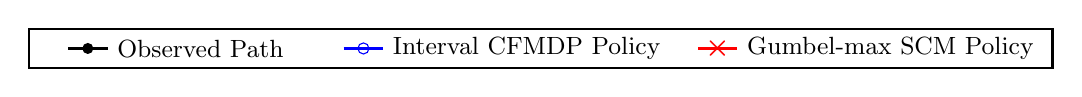
\begin{tikzpicture}[scale=1.0, every node/.style={scale=1.0}]
            \draw[thick, black] (-3, -0.25) rectangle (10, 0.25);
            %
            \draw[black, line width=1pt] (-2.5, 0.0) -- (-2,0.0);
            \fill[black] (-2.25,0.0) circle (2pt); %
            \node[right] at (-2,0.0) {\small Observed Path};
            
            %
            \draw[blue, line width=1pt] (1.0,0.0) -- (1.5,0.0);
            \node[draw=blue, circle, minimum size=4pt, inner sep=0pt] at (1.25,0.0) {}; %
            \node[right] at (1.5,0.0) {\small Interval CFMDP Policy};
            
            %
            \draw[red, line width=1pt] (5.5,0) -- (6,0);
            \node[red] at (5.75,0) {$\boldsymbol{\times}$}; %
            \node[right] at (6,0) {\small Gumbel-max SCM Policy};
        \end{tikzpicture}
    }\\
    %
    \subfigure[\footnotesize Lowest cumulative reward: Interval CFMDP ($312$), Gumbel-max SCM ($312$)]{%
        \resizebox{0.76\columnwidth}{!}{
             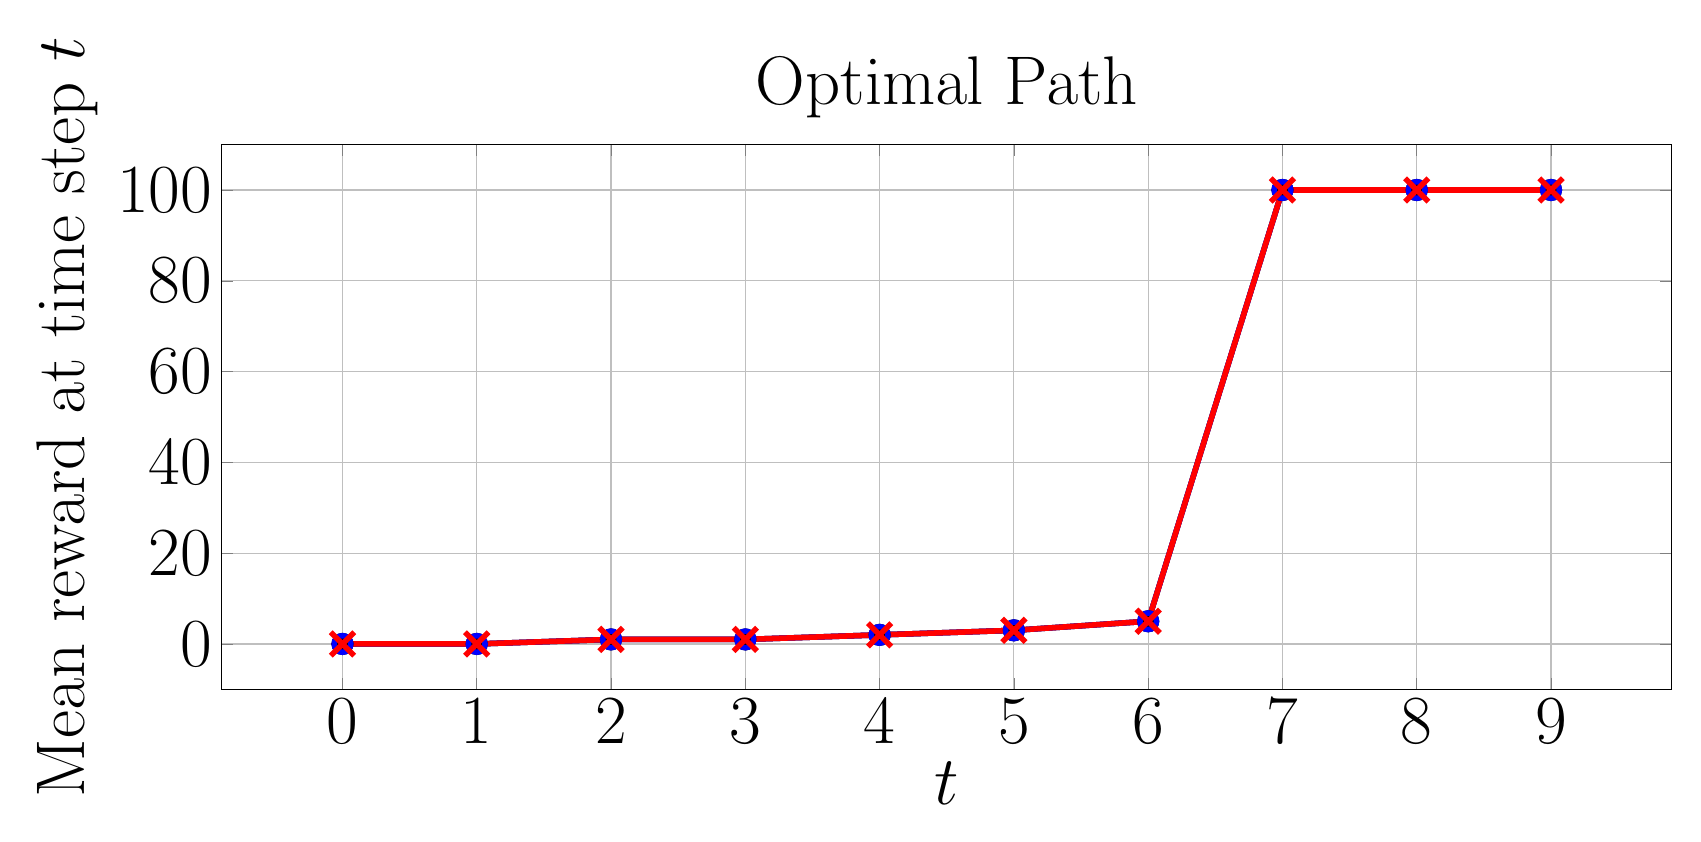
\begin{tikzpicture}
                \begin{axis}[
                    xlabel={$t$},
                    ylabel={Mean reward at time step $t$},
                    title={Optimal Path},
                    grid=both,
                    width=20cm, height=8.5cm,
                    every axis/.style={font=\Huge},
                    %
                ]
                \addplot[
                    color=black, %
                    mark=*, %
                    line width=2pt,
                    mark size=3pt,
                    error bars/.cd,
                    y dir=both, %
                    y explicit, %
                    error bar style={line width=1pt,solid},
                    error mark options={line width=1pt,mark size=4pt,rotate=90}
                ]
                coordinates {
                    (0, 0.0)  +- (0, 0.0)
                    (1, 0.0)  +- (0, 0.0) 
                    (2, 1.0)  +- (0, 0.0) 
                    (3, 1.0)  +- (0, 0.0)
                    (4, 2.0)  +- (0, 0.0)
                    (5, 3.0) +- (0, 0.0)
                    (6, 5.0) +- (0, 0.0)
                    (7, 100.0) +- (0, 0.0)
                    (8, 100.0) +- (0, 0.0)
                    (9, 100.0) +- (0, 0.0)
                };
                %
                \addplot[
                    color=blue, %
                    mark=o, %
                    line width=2pt,
                    mark size=3pt,
                    error bars/.cd,
                    y dir=both, %
                    y explicit, %
                    error bar style={line width=1pt,solid},
                    error mark options={line width=1pt,mark size=4pt,rotate=90}
                ]
                 coordinates {
                    (0, 0.0)  +- (0, 0.0)
                    (1, 0.0)  +- (0, 0.0) 
                    (2, 1.0)  +- (0, 0.0) 
                    (3, 1.0)  +- (0, 0.0)
                    (4, 2.0)  +- (0, 0.0)
                    (5, 3.0) +- (0, 0.0)
                    (6, 5.0) +- (0, 0.0)
                    (7, 100.0) +- (0, 0.0)
                    (8, 100.0) +- (0, 0.0)
                    (9, 100.0) +- (0, 0.0)
                };
                %
                \addplot[
                    color=red, %
                    mark=x, %
                    line width=2pt,
                    mark size=6pt,
                    error bars/.cd,
                    y dir=both, %
                    y explicit, %
                    error bar style={line width=1pt,solid},
                    error mark options={line width=1pt,mark size=4pt,rotate=90}
                ]
                coordinates {
                    (0, 0.0)  +- (0, 0.0)
                    (1, 0.0)  +- (0, 0.0) 
                    (2, 1.0)  +- (0, 0.0) 
                    (3, 1.0)  +- (0, 0.0)
                    (4, 2.0)  +- (0, 0.0)
                    (5, 3.0) +- (0, 0.0)
                    (6, 5.0) +- (0, 0.0)
                    (7, 100.0) +- (0, 0.0)
                    (8, 100.0) +- (0, 0.0)
                    (9, 100.0) +- (0, 0.0)
                };
                \end{axis}
            \end{tikzpicture}
         }
    }
    \hspace{1cm}
    \subfigure[\footnotesize Lowest cumulative reward: Interval CFMDP ($19$), Gumbel-max SCM ($-88$)]{%
         \resizebox{0.76\columnwidth}{!}{
            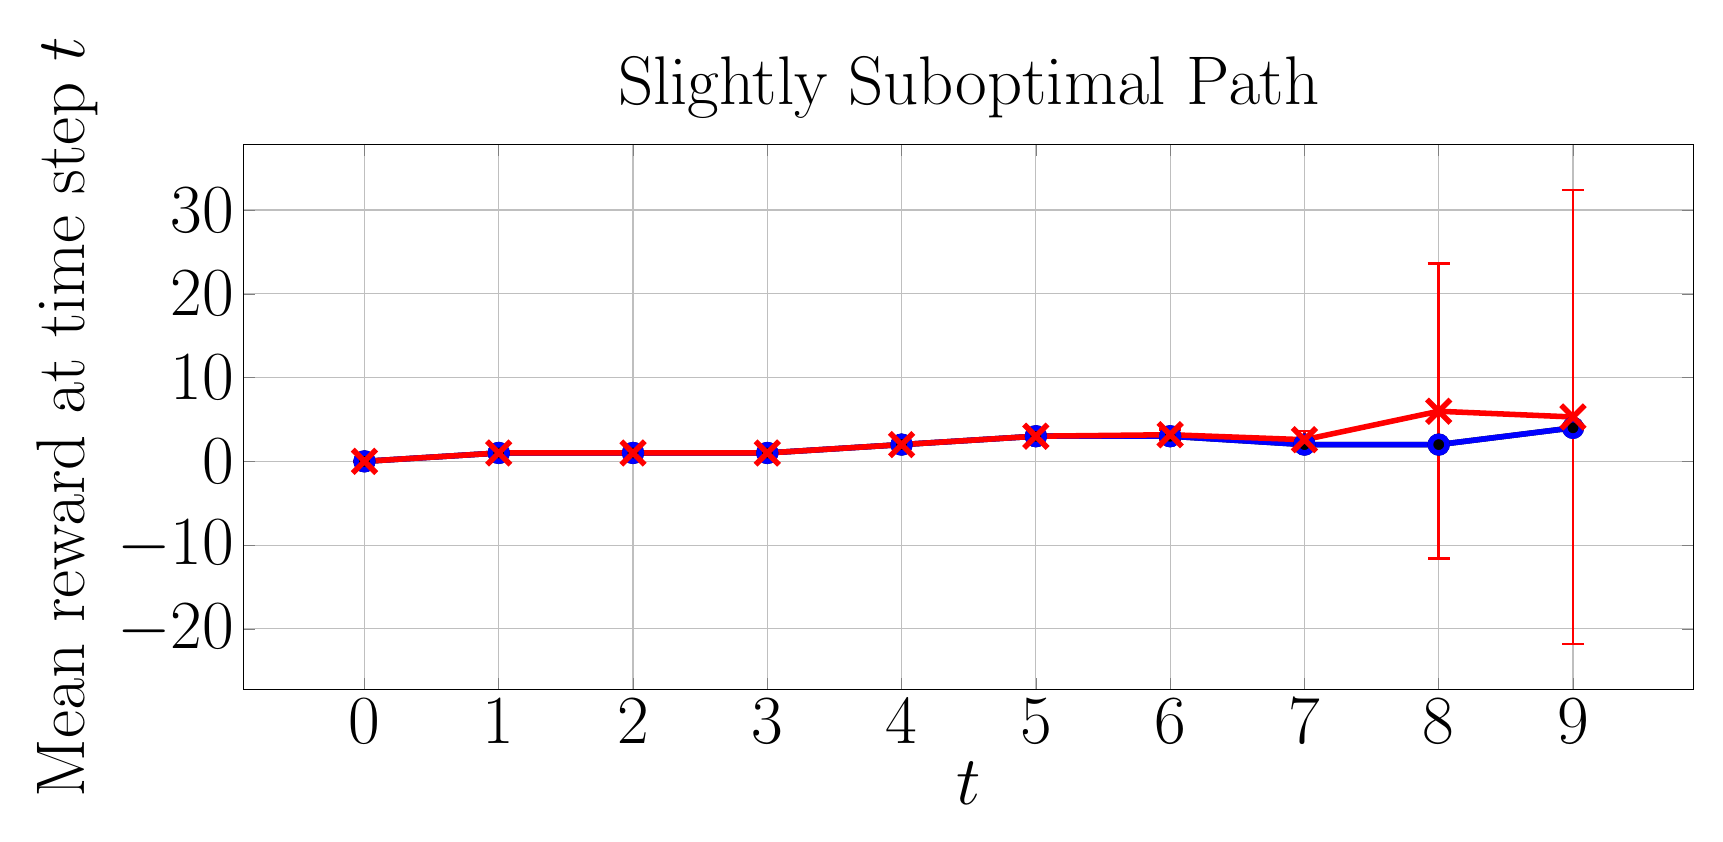
\begin{tikzpicture}
                \begin{axis}[
                    xlabel={$t$},
                    ylabel={Mean reward at time step $t$},
                    title={Slightly Suboptimal Path},
                    grid=both,
                    width=20cm, height=8.5cm,
                    every axis/.style={font=\Huge},
                    %
                ]
                \addplot[
                    color=black, %
                    mark=*, %
                    line width=2pt,
                    mark size=3pt,
                    error bars/.cd,
                    y dir=both, %
                    y explicit, %
                    error bar style={line width=1pt,solid},
                    error mark options={line width=1pt,mark size=4pt,rotate=90}
                ]
              coordinates {
                    (0, 0.0)  +- (0, 0.0)
                    (1, 1.0)  +- (0, 0.0) 
                    (2, 1.0)  +- (0, 0.0) 
                    (3, 1.0)  +- (0, 0.0)
                    (4, 2.0)  +- (0, 0.0)
                    (5, 3.0) +- (0, 0.0)
                    (6, 3.0) +- (0, 0.0)
                    (7, 2.0) +- (0, 0.0)
                    (8, 2.0) +- (0, 0.0)
                    (9, 4.0) +- (0, 0.0)
                };
                %
                \addplot[
                    color=blue, %
                    mark=o, %
                    line width=2pt,
                    mark size=3pt,
                    error bars/.cd,
                    y dir=both, %
                    y explicit, %
                    error bar style={line width=1pt,solid},
                    error mark options={line width=1pt,mark size=4pt,rotate=90}
                ]
              coordinates {
                    (0, 0.0)  +- (0, 0.0)
                    (1, 1.0)  +- (0, 0.0) 
                    (2, 1.0)  +- (0, 0.0) 
                    (3, 1.0)  +- (0, 0.0)
                    (4, 2.0)  +- (0, 0.0)
                    (5, 3.0) +- (0, 0.0)
                    (6, 3.0) +- (0, 0.0)
                    (7, 2.0) +- (0, 0.0)
                    (8, 2.0) +- (0, 0.0)
                    (9, 4.0) +- (0, 0.0)
                };
                %
                \addplot[
                    color=red, %
                    mark=x, %
                    line width=2pt,
                    mark size=6pt,
                    error bars/.cd,
                    y dir=both, %
                    y explicit, %
                    error bar style={line width=1pt,solid},
                    error mark options={line width=1pt,mark size=4pt,rotate=90}
                ]
                coordinates {
                    (0, 0.0)  +- (0, 0.0)
                    (1, 1.0)  +- (0, 0.0) 
                    (2, 1.0)  +- (0, 0.0) 
                    (3, 1.0)  +- (0, 0.0)
                    (4, 2.0)  += (0, 0.0)
                    (5, 3.0)  += (0, 0.0)
                    (6, 3.17847) += (0, 0.62606746) -= (0, 0.62606746)
                    (7, 2.5832885) += (0, 1.04598233) -= (0, 1.04598233)
                    (8, 5.978909) += (0, 17.60137623) -= (0, 17.60137623)
                    (9, 5.297059) += (0, 27.09227512) -= (0, 27.09227512)
                };
                \end{axis}
            \end{tikzpicture}
         }
    }\\[-1.5pt]
    \subfigure[\footnotesize Lowest cumulative reward: Interval CFMDP ($14$), Gumbel-max SCM ($-598$)]{%
         \resizebox{0.76\columnwidth}{!}{
             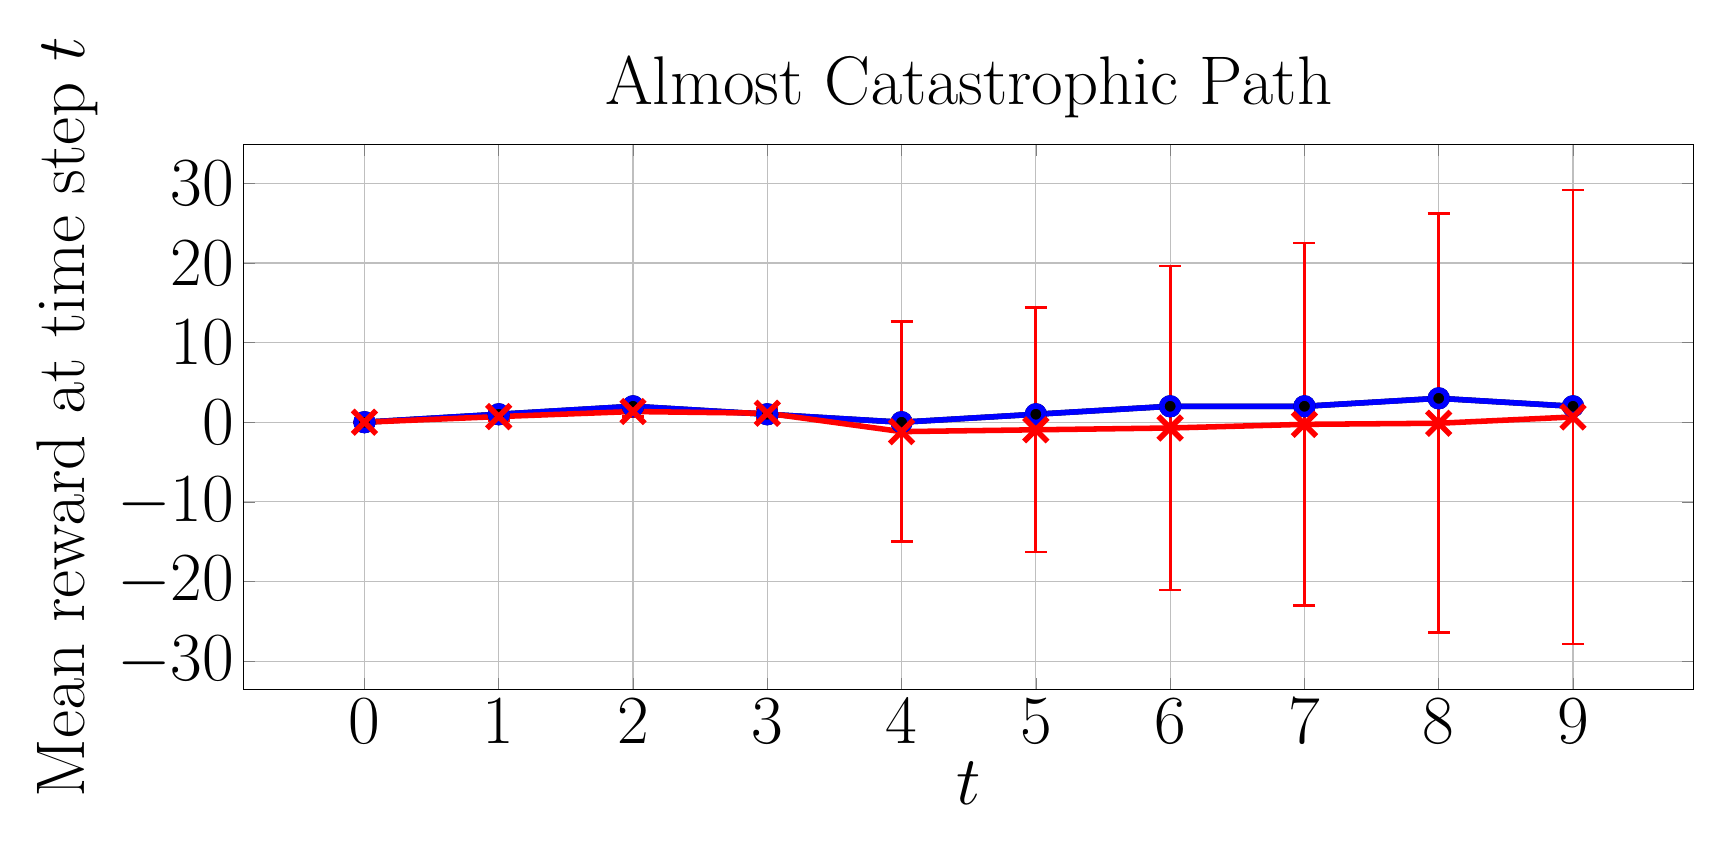
\begin{tikzpicture}
                \begin{axis}[
                    xlabel={$t$},
                    ylabel={Mean reward at time step $t$},
                    title={Almost Catastrophic Path},
                    grid=both,
                    width=20cm, height=8.5cm,
                    every axis/.style={font=\Huge},
                    %
                ]
                \addplot[
                    color=black, %
                    mark=*, %
                    line width=2pt,
                    mark size=3pt,
                    error bars/.cd,
                    y dir=both, %
                    y explicit, %
                    error bar style={line width=1pt,solid},
                    error mark options={line width=1pt,mark size=4pt,rotate=90}
                ]
                coordinates {
                    (0, 0.0)  +- (0, 0.0)
                    (1, 1.0)  +- (0, 0.0) 
                    (2, 2.0)  +- (0, 0.0) 
                    (3, 1.0)  +- (0, 0.0)
                    (4, 0.0)  +- (0, 0.0)
                    (5, 1.0) +- (0, 0.0)
                    (6, 2.0) +- (0, 0.0)
                    (7, 2.0) +- (0, 0.0)
                    (8, 3.0) +- (0, 0.0)
                    (9, 2.0) +- (0, 0.0)
                };
                %
                \addplot[
                    color=blue, %
                    mark=o, %
                    line width=2pt,
                    mark size=3pt,
                    error bars/.cd,
                    y dir=both, %
                    y explicit, %
                    error bar style={line width=1pt,solid},
                    error mark options={line width=1pt,mark size=4pt,rotate=90}
                ]
                coordinates {
                    (0, 0.0)  +- (0, 0.0)
                    (1, 1.0)  +- (0, 0.0) 
                    (2, 2.0)  +- (0, 0.0) 
                    (3, 1.0)  +- (0, 0.0)
                    (4, 0.0)  +- (0, 0.0)
                    (5, 1.0) +- (0, 0.0)
                    (6, 2.0) +- (0, 0.0)
                    (7, 2.0) +- (0, 0.0)
                    (8, 3.0) +- (0, 0.0)
                    (9, 2.0) +- (0, 0.0)
                };
                %
                \addplot[
                    color=red, %
                    mark=x, %
                    line width=2pt,
                    mark size=6pt,
                    error bars/.cd,
                    y dir=both, %
                    y explicit, %
                    error bar style={line width=1pt,solid},
                    error mark options={line width=1pt,mark size=4pt,rotate=90}
                ]
                coordinates {
                    (0, 0.0)  +- (0, 0.0)
                    (1, 0.7065655)  +- (0, 0.4553358) 
                    (2, 1.341673)  +- (0, 0.67091621) 
                    (3, 1.122926)  +- (0, 0.61281824)
                    (4, -1.1821935)  +- (0, 13.82444042)
                    (5, -0.952399)  +- (0, 15.35195457)
                    (6, -0.72672) +- (0, 20.33508414)
                    (7, -0.268983) +- (0, 22.77861454)
                    (8, -0.1310835) +- (0, 26.31013314)
                    (9, 0.65806) +- (0, 28.50670214)
                };
                %
            %
            %
            %
            %
            %
            %
            %
            %
            %
            %
            %
            %
            %
            %
            %
            %
            %
            %
                \end{axis}
            \end{tikzpicture}
         }
    }
    \hspace{1cm}
    \subfigure[\footnotesize Lowest cumulative reward: Interval CFMDP ($-698$), Gumbel-max SCM ($-698$)]{%
         \resizebox{0.76\columnwidth}{!}{
            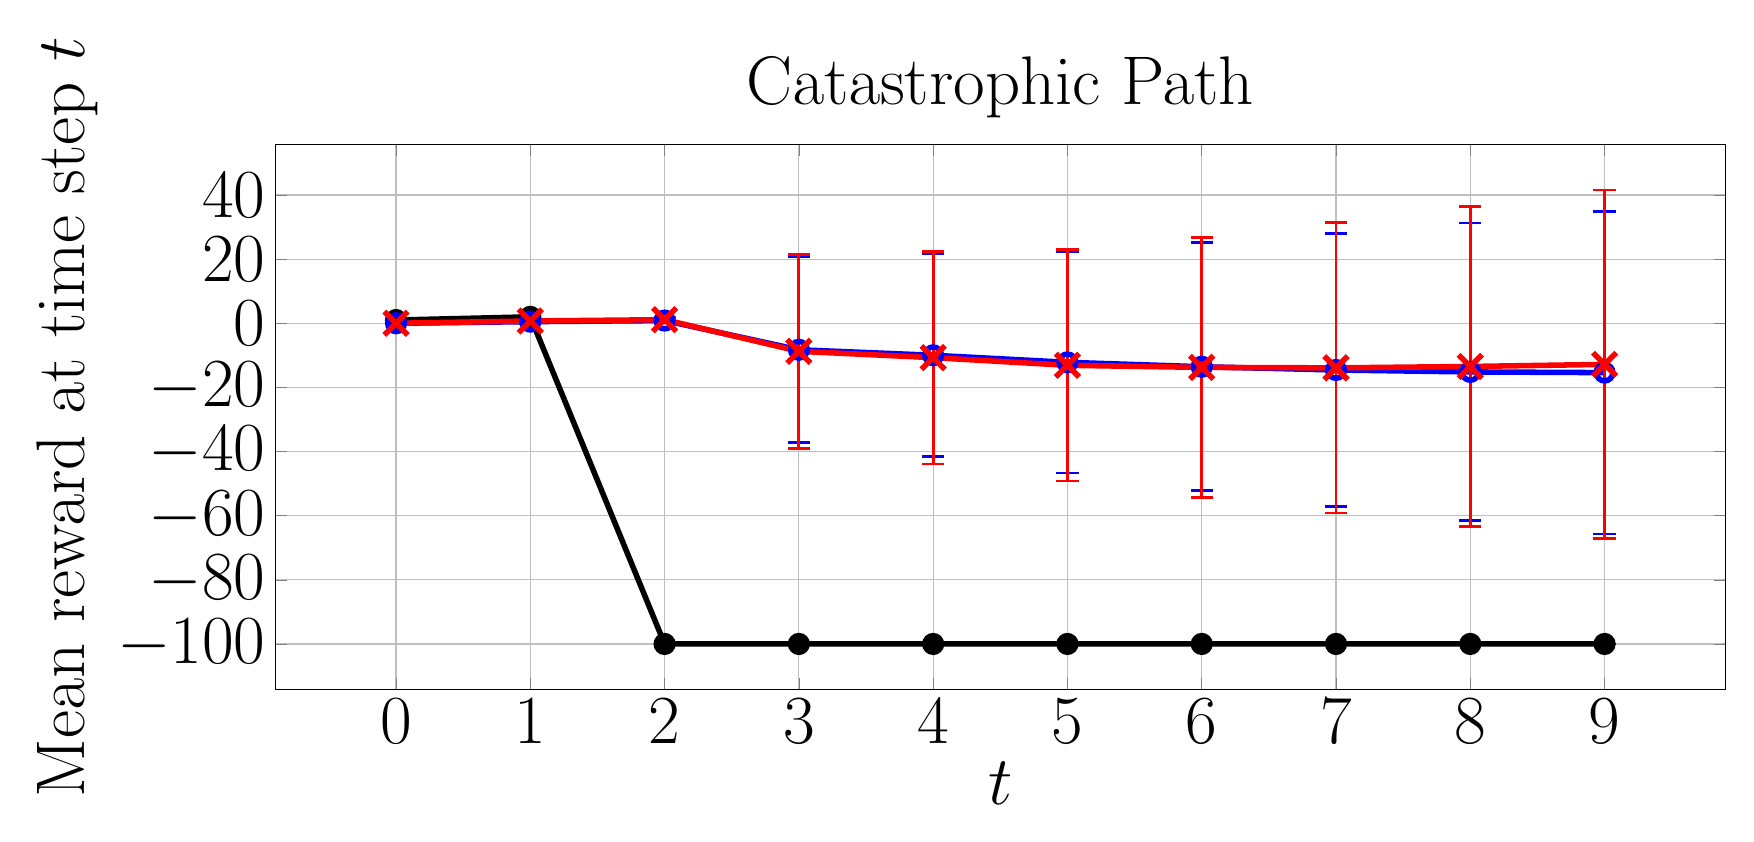
\begin{tikzpicture}
                \begin{axis}[
                    xlabel={$t$},
                    ylabel={Mean reward at time step $t$},
                    title={Catastrophic Path},
                    grid=both,
                    width=20cm, height=8.5cm,
                    every axis/.style={font=\Huge},
                    %
                ]
                \addplot[
                    color=black, %
                    mark=*, %
                    line width=2pt,
                    mark size=3pt,
                    error bars/.cd,
                    y dir=both, %
                    y explicit, %
                    error bar style={line width=1pt,solid},
                    error mark options={line width=1pt,mark size=4pt,rotate=90}
                ]
                coordinates {
                    (0, 1.0)  +- (0, 0.0)
                    (1, 2.0)  +- (0, 0.0) 
                    (2, -100.0)  +- (0, 0.0) 
                    (3, -100.0)  +- (0, 0.0)
                    (4, -100.0)  +- (0, 0.0)
                    (5, -100.0) +- (0, 0.0)
                    (6, -100.0) +- (0, 0.0)
                    (7, -100.0) +- (0, 0.0)
                    (8, -100.0) +- (0, 0.0)
                    (9, -100.0) +- (0, 0.0)
                };
                %
                \addplot[
                    color=blue, %
                    mark=o, %
                    line width=2pt,
                    mark size=3pt,
                    error bars/.cd,
                    y dir=both, %
                    y explicit, %
                    error bar style={line width=1pt,solid},
                    error mark options={line width=1pt,mark size=4pt,rotate=90}
                ]
                coordinates {
                    (0, 0.0)  +- (0, 0.0)
                    (1, 0.504814)  +- (0, 0.49997682) 
                    (2, 0.8439835)  +- (0, 0.76831917) 
                    (3, -8.2709165)  +- (0, 28.93656754)
                    (4, -9.981082)  +- (0, 31.66825363)
                    (5, -12.1776325) +- (0, 34.53463233)
                    (6, -13.556076) +- (0, 38.62845372)
                    (7, -14.574418) +- (0, 42.49603359)
                    (8, -15.1757075) +- (0, 46.41913968)
                    (9, -15.3900395) +- (0, 50.33563368)
                };
                %
                \addplot[
                    color=red, %
                    mark=x, %
                    line width=2pt,
                    mark size=6pt,
                    error bars/.cd,
                    y dir=both, %
                    y explicit, %
                    error bar style={line width=1pt,solid},
                    error mark options={line width=1pt,mark size=4pt,rotate=90}
                ]
                coordinates {
                    (0, 0.0)  +- (0, 0.0)
                    (1, 0.701873)  +- (0, 0.45743556) 
                    (2, 1.1227805)  +- (0, 0.73433129) 
                    (3, -8.7503255)  +- (0, 30.30257976)
                    (4, -10.722092)  +- (0, 33.17618589)
                    (5, -13.10721)  +- (0, 36.0648089)
                    (6, -13.7631645) +- (0, 40.56553451)
                    (7, -13.909043) +- (0, 45.23829402)
                    (8, -13.472517) +- (0, 49.96270296)
                    (9, -12.8278835) +- (0, 54.38618735)
                };
                %
            %
            %
            %
            %
            %
            %
            %
            %
            %
            %
            %
            %
            %
            %
            %
            %
            %
            %
                \end{axis}
            \end{tikzpicture}
         }
    }
    \caption{Average instant reward of CF paths induced by policies on GridWorld $p=0.4$.}
    \label{fig: reward p=0.4}
\end{figure*}

\subsection{Experimental Setup}
To compare policy performance, we measure the average rewards of counterfactual paths induced by our policy and the Gumbel-max policy by uniformly sampling $200$ counterfactual MDPs from the ICFMDP and generating $10,000$ counterfactual paths over each sampled CFMDP. \jl{Since the interval CFMDP depends on the observed path, we select $4$  paths of varying optimality to evaluate how the observed path impacts the performance of both policies: an optimal path, a slightly suboptimal path that could reach the optimal reward with a few changes, a catastrophic path that enters a catastrophic, terminal state with low reward, and an almost catastrophic path that was close to entering a catastrophic state.} When measuring the average probability bound widths and execution time needed to generate the ICFMDPs, we averaged over $20$ randomly generated observed paths
\footnote{Further training details are provided in Appendix \ref{app: training details}, and the code is provided at \href{https://github.com/ddv-lab/robust-cf-inference-in-MDPs}{https://github.com/ddv-lab/robust-cf-inference-in-MDPs}
%
%
.}.

\subsection{GridWorld}
\jl{The GridWorld MDP is a $4 \times 4$ grid where an agent must navigate from the top-left corner to the goal state in the bottom-right corner, avoiding a dangerous terminal state in the centre. At each time step, the agent can move up, down, left, or right, but there is a small probability (controlled by hyper-parameter $p$) of moving in an unintended direction. As the agent nears the goal, the reward for each state increases, culminating in a reward of $+100$ for reaching the goal. Entering the dangerous state results in a penalty of $-100$. We use two versions of GridWorld: a less stochastic version with $p=0.9$ (i.e., $90$\% chance of moving in the chosen direction) and a more stochastic version with $p=0.4$.}

\paragraph{GridWorld ($p=0.9$)}
When $p=0.9$, the counterfactual probability bounds are typically narrow (see Table \ref{tab:nonzero_probs} for average measurements). Consequently, as shown in Figure \ref{fig: reward p=0.9}, both policies are nearly identical and perform similarly well across the optimal, slightly suboptimal, and catastrophic paths.
%
However, for the almost catastrophic path, the interval CFMDP path is more conservative and follows the observed path more closely (as this is where the probability bounds are narrowest), which typically requires one additional step to reach the goal state than the Gumbel-max SCM policy.
%

\paragraph{GridWorld ($p=0.4$)}
\jl{When $p=0.4$, the GridWorld environment becomes more uncertain, increasing the risk of entering the dangerous state even if correct actions are chosen. Thus, as shown in Figure \ref{fig: reward p=0.4}, the interval CFMDP policy adopts a more conservative approach, avoiding deviation from the observed policy if it cannot guarantee higher counterfactual rewards (see the slightly suboptimal and almost catastrophic paths), whereas the Gumbel-max SCM is inconsistent: it can yield higher rewards, but also much lower rewards, reflected in the wide error bars.} For the catastrophic path, both policies must deviate from the observed path to achieve a higher reward and, in this case, perform similarly.
%
%
%
%
\subsection{Sepsis}
The Sepsis MDP \citep{oberst2019counterfactual} simulates trajectories of Sepsis patients. Each state consists of four vital signs (heart rate, blood pressure, oxygen concentration, and glucose levels), categorised as low, normal, or high.
and three treatments that can be toggled on/off at each time step (8 actions in total). Unlike \citet{oberst2019counterfactual}, we scale rewards based on the number of out-of-range vital signs, between $-1000$ (patient dies) and $1000$ (patient discharged). \jl{Like the GridWorld $p=0.4$ experiment, the Sepsis MDP is highly uncertain, as many states are equally likely to lead to optimal and poor outcomes. Thus, as shown in Figure \ref{fig: reward sepsis}, both policies follow the observed optimal and almost catastrophic paths to guarantee rewards are no worse than the observation.} However, improving the catastrophic path requires deviating from the observation. Here, the Gumbel-max SCM policy, on average, performs better than the interval CFMDP policy. But, since both policies have lower bounds clipped at $-1000$, neither policy reliably improves over the observation. In contrast, for the slightly suboptimal path, the interval CFMDP policy performs significantly better, shown by its higher lower bounds. 
Moreover, in these two cases, the worst-case counterfactual path generated by the interval CFMDP policy is better than that of the Gumbel-max SCM policy,
indicating its greater robustness.
%
\begin{figure*}
    \centering
     \resizebox{0.6\textwidth}{!}{
        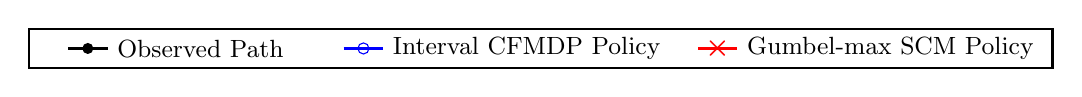
\begin{tikzpicture}[scale=1.0, every node/.style={scale=1.0}]
            \draw[thick, black] (-3, -0.25) rectangle (10, 0.25);
            %
            \draw[black, line width=1pt] (-2.5, 0.0) -- (-2,0.0);
            \fill[black] (-2.25,0.0) circle (2pt); %
            \node[right] at (-2,0.0) {\small Observed Path};
            
            %
            \draw[blue, line width=1pt] (1.0,0.0) -- (1.5,0.0);
            \node[draw=blue, circle, minimum size=4pt, inner sep=0pt] at (1.25,0.0) {}; %
            \node[right] at (1.5,0.0) {\small Interval CFMDP Policy};
            
            %
            \draw[red, line width=1pt] (5.5,0) -- (6,0);
            \node[red] at (5.75,0) {$\boldsymbol{\times}$}; %
            \node[right] at (6,0) {\small Gumbel-max SCM Policy};
        \end{tikzpicture}
    }\\
    \subfigure[\footnotesize Lowest cumulative reward: Interval CFMDP ($8000$), Gumbel-max SCM ($8000$)]{%
         \resizebox{0.76\columnwidth}{!}{
             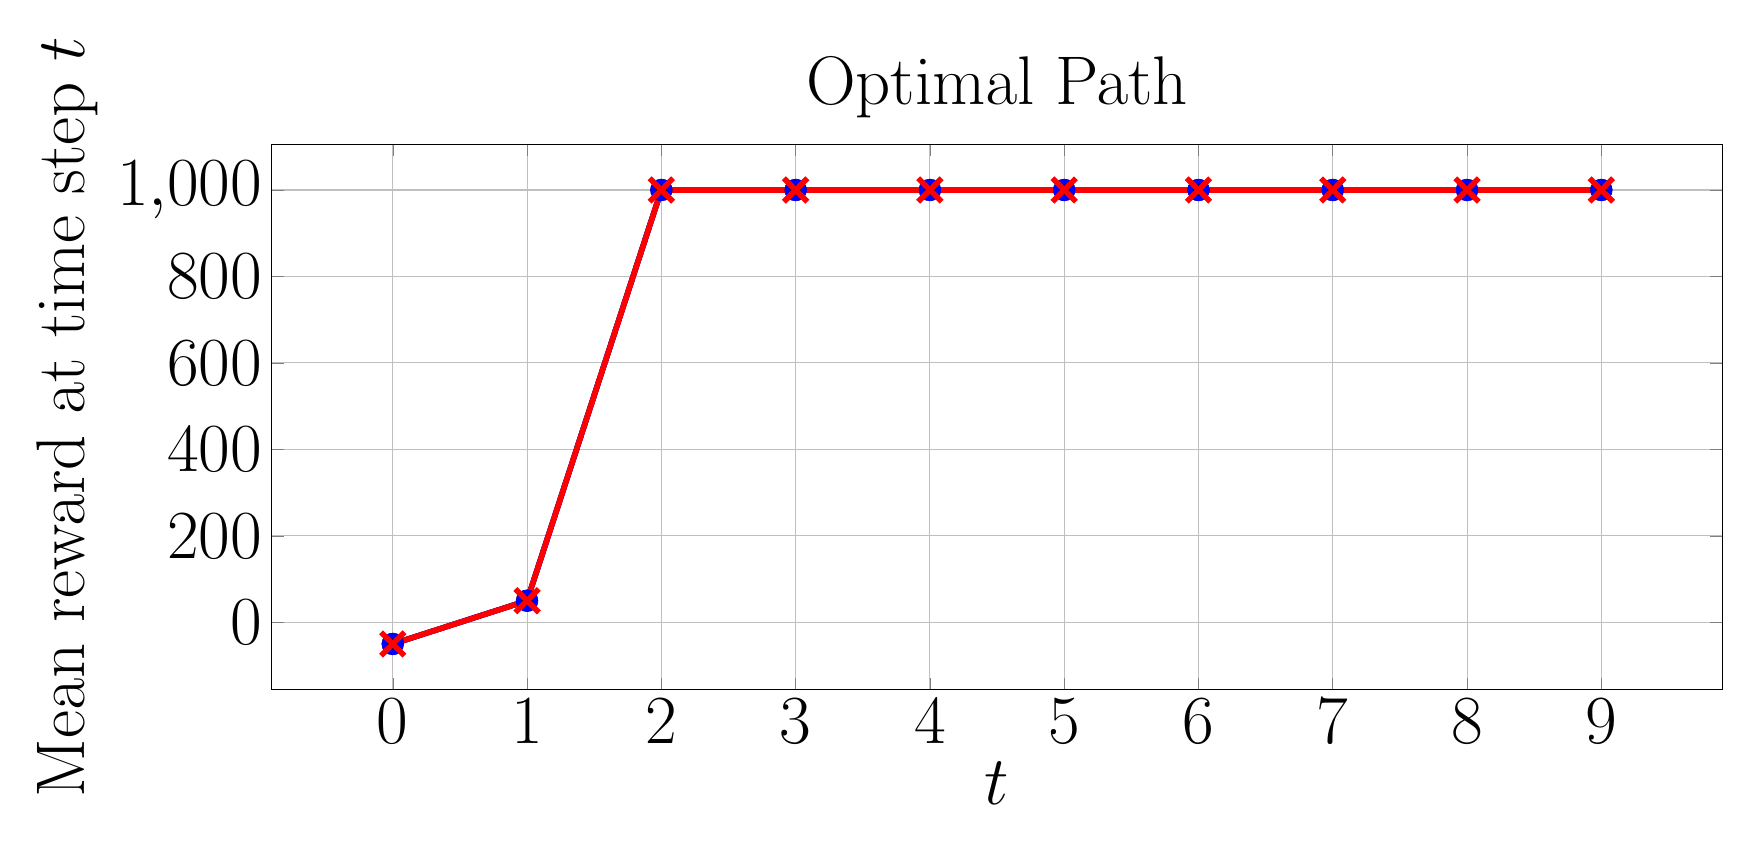
\begin{tikzpicture}
                \begin{axis}[
                    xlabel={$t$},
                    ylabel={Mean reward at time step $t$},
                    title={Optimal Path},
                    grid=both,
                    width=20cm, height=8.5cm,
                    every axis/.style={font=\Huge},
                    %
                ]
                \addplot[
                    color=black, %
                    mark=*, %
                    line width=2pt,
                    mark size=3pt,
                ]
                coordinates {
                    (0, -50.0)
                    (1, 50.0)
                    (2, 1000.0)
                    (3, 1000.0)
                    (4, 1000.0)
                    (5, 1000.0)
                    (6, 1000.0)
                    (7, 1000.0)
                    (8, 1000.0)
                    (9, 1000.0)
                };
                %
                \addplot[
                    color=blue, %
                    mark=o, %
                    line width=2pt,
                    mark size=3pt,
                    error bars/.cd,
                    y dir=both, %
                    y explicit, %
                    error bar style={line width=1pt,solid},
                    error mark options={line width=1pt,mark size=4pt,rotate=90}
                ]
                coordinates {
                    (0, -50.0)  +- (0, 0.0)
                    (1, 50.0)  +- (0, 0.0) 
                    (2, 1000.0)  +- (0, 0.0) 
                    (3, 1000.0)  +- (0, 0.0)
                    (4, 1000.0)  +- (0, 0.0)
                    (5, 1000.0) +- (0, 0.0)
                    (6, 1000.0) +- (0, 0.0)
                    (7, 1000.0) +- (0, 0.0)
                    (8, 1000.0) +- (0, 0.0)
                    (9, 1000.0) +- (0, 0.0)
                };
                %
                \addplot[
                    color=red, %
                    mark=x, %
                    line width=2pt,
                    mark size=6pt,
                    error bars/.cd,
                    y dir=both, %
                    y explicit, %
                    error bar style={line width=1pt,solid},
                    error mark options={line width=1pt,mark size=4pt,rotate=90}
                ]
                coordinates {
                    (0, -50.0)  +- (0, 0.0)
                    (1, 50.0)  +- (0, 0.0) 
                    (2, 1000.0)  +- (0, 0.0) 
                    (3, 1000.0)  +- (0, 0.0)
                    (4, 1000.0)  +- (0, 0.0)
                    (5, 1000.0) +- (0, 0.0)
                    (6, 1000.0) +- (0, 0.0)
                    (7, 1000.0) +- (0, 0.0)
                    (8, 1000.0) +- (0, 0.0)
                    (9, 1000.0) +- (0, 0.0)
                };
                %
                \end{axis}
            \end{tikzpicture}
         }
    }
    \hspace{1cm}
    \subfigure[\footnotesize Lowest cumulative reward: Interval CFMDP ($-5980$), Gumbel-max SCM ($-8000$)]{%
         \resizebox{0.76\columnwidth}{!}{
            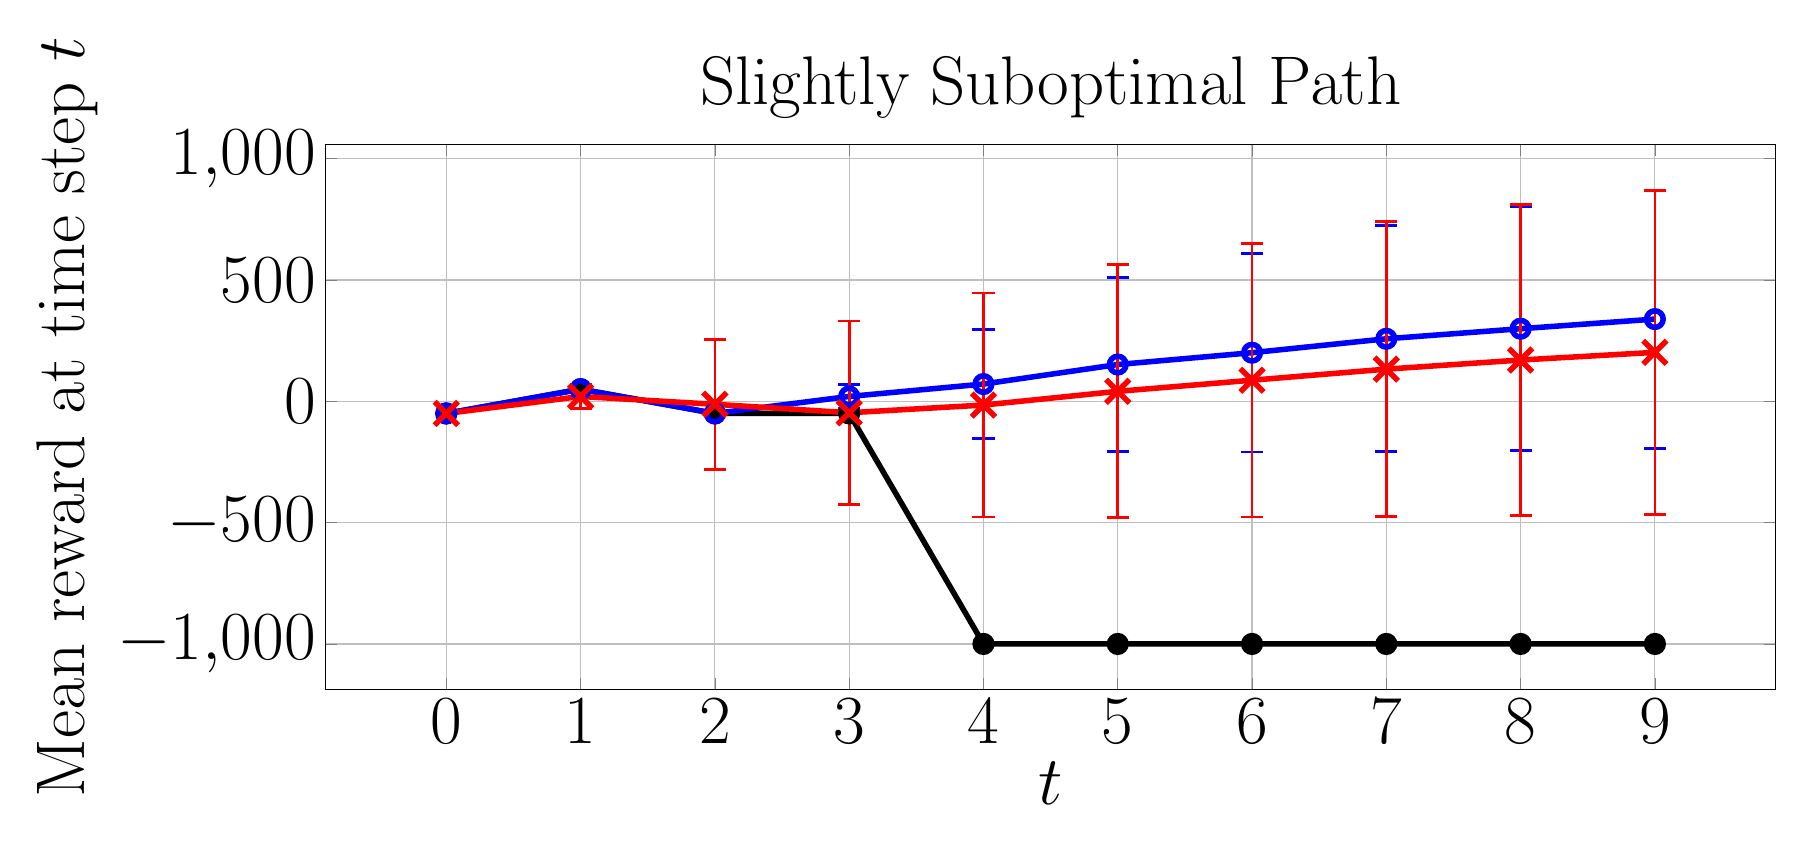
\begin{tikzpicture}
                \begin{axis}[
                    xlabel={$t$},
                    ylabel={Mean reward at time step $t$},
                    title={Slightly Suboptimal Path},
                    grid=both,
                    width=20cm, height=8.5cm,
                    every axis/.style={font=\Huge},
                    %
                ]
               \addplot[
                    color=black, %
                    mark=*, %
                    line width=2pt,
                    mark size=3pt,
                ]
                coordinates {
                    (0, -50.0)
                    (1, 50.0)
                    (2, -50.0)
                    (3, -50.0)
                    (4, -1000.0)
                    (5, -1000.0)
                    (6, -1000.0)
                    (7, -1000.0)
                    (8, -1000.0)
                    (9, -1000.0)
                };
                %
                \addplot[
                    color=blue, %
                    mark=o, %
                    line width=2pt,
                    mark size=3pt,
                    error bars/.cd,
                    y dir=both, %
                    y explicit, %
                    error bar style={line width=1pt,solid},
                    error mark options={line width=1pt,mark size=4pt,rotate=90}
                ]
                coordinates {
                    (0, -50.0)  +- (0, 0.0)
                    (1, 50.0)  +- (0, 0.0) 
                    (2, -50.0)  +- (0, 0.0) 
                    (3, 20.0631)  +- (0, 49.97539413)
                    (4, 71.206585)  +- (0, 226.02033693)
                    (5, 151.60797) +- (0, 359.23292559)
                    (6, 200.40593) +- (0, 408.86185176)
                    (7, 257.77948) +- (0, 466.10372804)
                    (8, 299.237465) +- (0, 501.82579506)
                    (9, 338.9129) +- (0, 532.06124996)
                };
                %
                \addplot[
                    color=red, %
                    mark=x, %
                    line width=2pt,
                    mark size=6pt,
                    error bars/.cd,
                    y dir=both, %
                    y explicit, %
                    error bar style={line width=1pt,solid},
                    error mark options={line width=1pt,mark size=4pt,rotate=90}
                ]
                coordinates {
                    (0, -50.0)  +- (0, 0.0)
                    (1, 20.00736)  +- (0, 49.99786741) 
                    (2, -12.282865)  +- (0, 267.598755) 
                    (3, -47.125995)  +- (0, 378.41755832)
                    (4, -15.381965)  +- (0, 461.77616558)
                    (5, 41.15459) +- (0, 521.53189262)
                    (6, 87.01595) +- (0, 564.22243126 )
                    (7, 132.62376) +- (0, 607.31338037)
                    (8, 170.168145) +- (0, 641.48013693)
                    (9, 201.813135) +- (0, 667.29441777)
                };
                %
                %
                %
                %
                %
                %
                %
                %
                %
                %
                %
                %
                %
                %
                %
                %
                %
                %
                %
                \end{axis}
            \end{tikzpicture}
         }
    }\\[-1.5pt]
    \subfigure[\footnotesize Lowest cumulative reward: Interval CFMDP ($100$), Gumbel-max SCM ($100$)]{%
         \resizebox{0.76\columnwidth}{!}{
             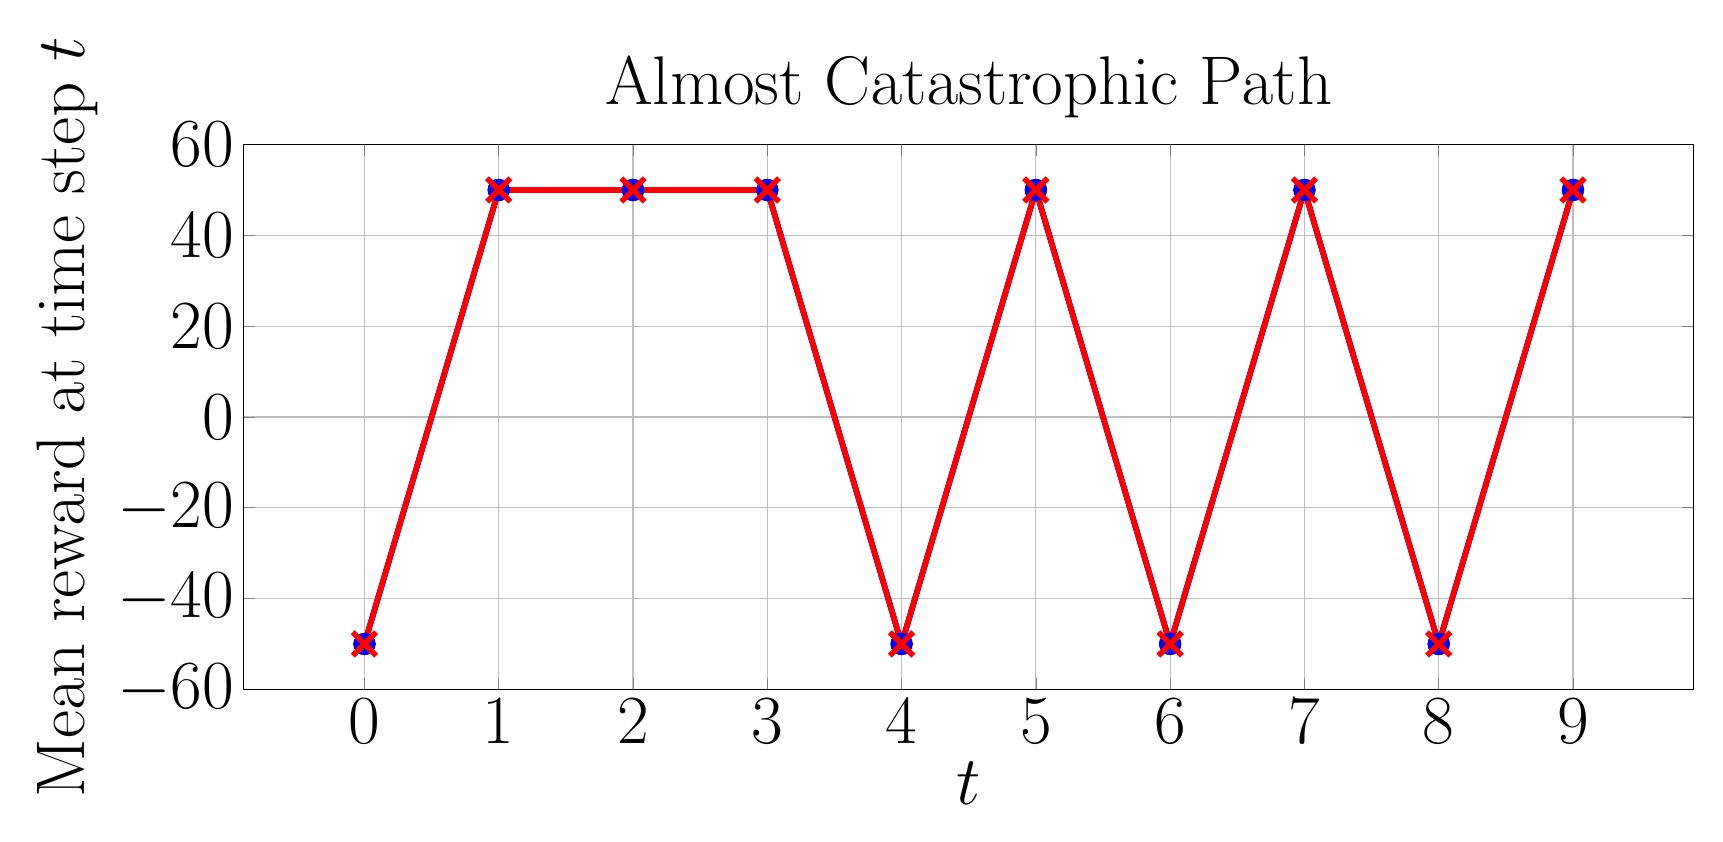
\begin{tikzpicture}
                \begin{axis}[
                    xlabel={$t$},
                    ylabel={Mean reward at time step $t$},
                    title={Almost Catastrophic Path},
                    grid=both,
                    every axis/.style={font=\Huge},
                    width=20cm, height=8.5cm,
                    %
                ]
               \addplot[
                    color=black, %
                    mark=*, %
                    line width=2pt,
                    mark size=3pt,
                ]
                coordinates {
                    (0, -50.0)
                    (1, 50.0)
                    (2, 50.0)
                    (3, 50.0)
                    (4, -50.0)
                    (5, 50.0)
                    (6, -50.0)
                    (7, 50.0)
                    (8, -50.0)
                    (9, 50.0)
                };
                %
                %
                \addplot[
                    color=blue, %
                    mark=o, %
                    line width=2pt,
                    mark size=3pt,
                    error bars/.cd,
                    y dir=both, %
                    y explicit, %
                    error bar style={line width=1pt,solid},
                    error mark options={line width=1pt,mark size=4pt,rotate=90}
                ]
                coordinates {
                    (0, -50.0)  +- (0, 0.0)
                    (1, 50.0)  +- (0, 0.0) 
                    (2, 50.0)  +- (0, 0.0) 
                    (3, 50.0)  +- (0, 0.0)
                    (4, -50.0)  +- (0, 0.0)
                    (5, 50.0) +- (0, 0.0)
                    (6, -50.0) +- (0, 0.0)
                    (7, 50.0) +- (0, 0.0)
                    (8, -50.0) +- (0, 0.0)
                    (9, 50.0) +- (0, 0.0)
                };
                %
                \addplot[
                    color=red, %
                    mark=x, %
                    line width=2pt,
                    mark size=6pt,
                    error bars/.cd,
                    y dir=both, %
                    y explicit, %
                    error bar style={line width=1pt,solid},
                    error mark options={line width=1pt,mark size=4pt,rotate=90}
                ]
                coordinates {
                    (0, -50.0)  +- (0, 0.0)
                    (1, 50.0)  +- (0, 0.0) 
                    (2, 50.0)  +- (0, 0.0) 
                    (3, 50.0)  +- (0, 0.0)
                    (4, -50.0)  +- (0, 0.0)
                    (5, 50.0) +- (0, 0.0)
                    (6, -50.0) +- (0, 0.0)
                    (7, 50.0) +- (0, 0.0)
                    (8, -50.0) +- (0, 0.0)
                    (9, 50.0) +- (0, 0.0)
                };
                %
                %
                %
                %
                %
                %
                %
                %
                %
                %
                %
                %
                %
                %
                %
                %
                %
                %
                %
                \end{axis}
            \end{tikzpicture}
         }
    }
    \hspace{1cm}
    \subfigure[\footnotesize Lowest cumulative reward: Interval CFMDP ($-7150$), Gumbel-max SCM ($-9050$)]{%
         \resizebox{0.76\columnwidth}{!}{
            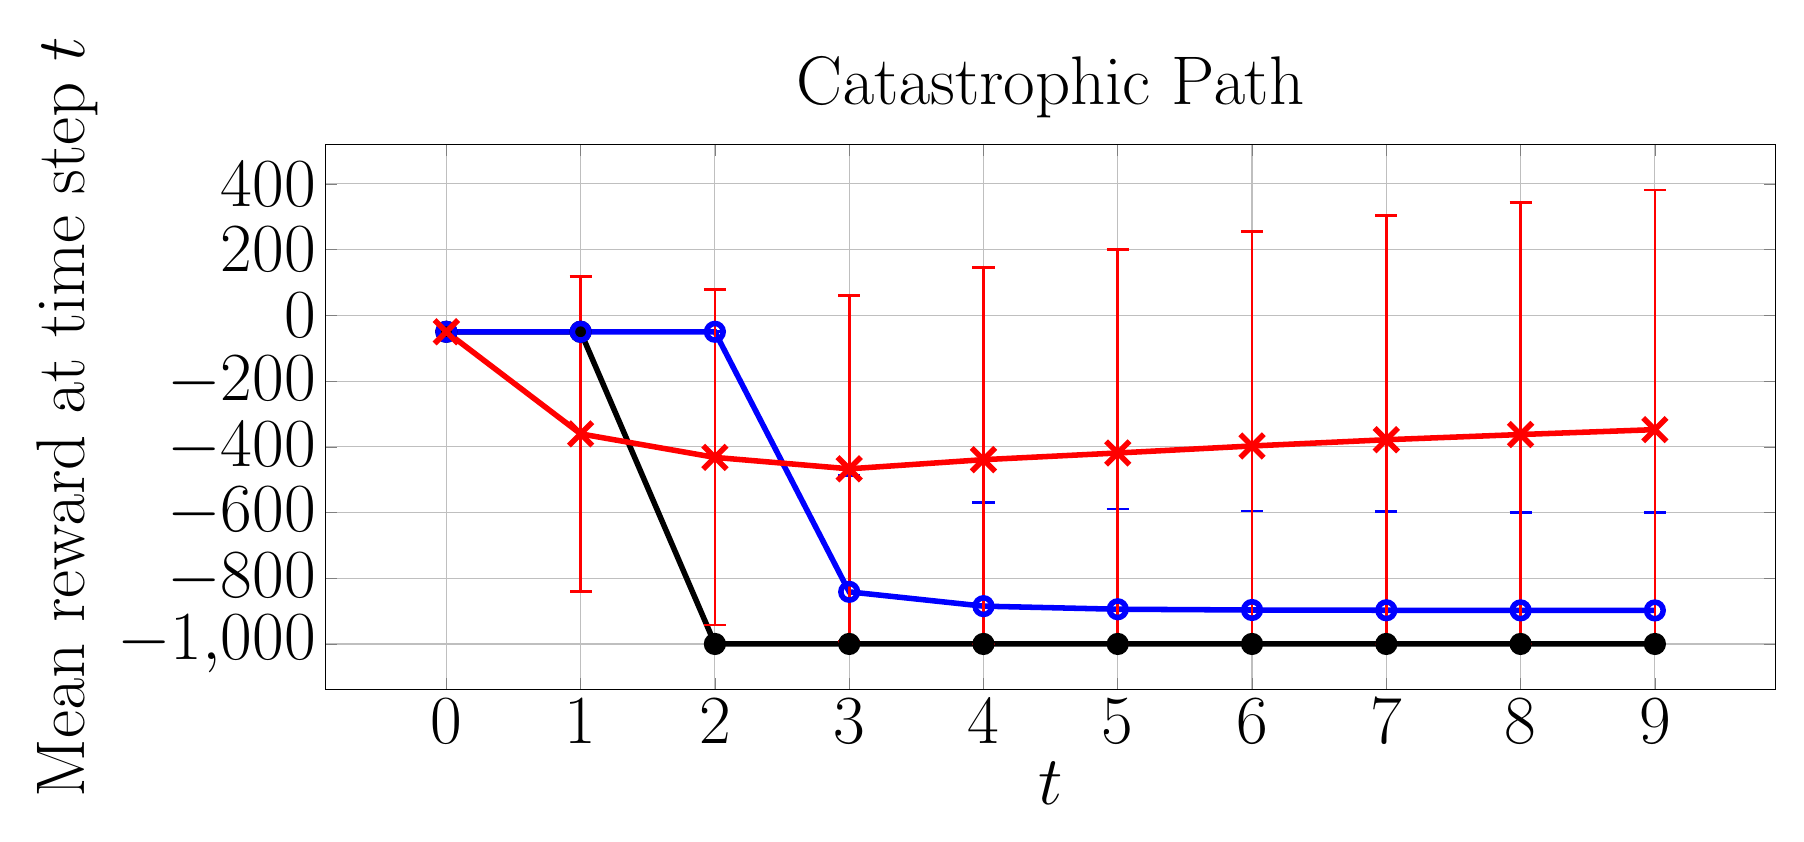
\begin{tikzpicture}
                \begin{axis}[
                    xlabel={$t$},
                    ylabel={Mean reward at time step $t$},
                    title={Catastrophic Path},
                    grid=both,
                    width=20cm, height=8.5cm,
                    every axis/.style={font=\Huge},
                    %
                ]
               \addplot[
                    color=black, %
                    mark=*, %
                    line width=2pt,
                    mark size=3pt,
                ]
                coordinates {
                    (0, -50.0)
                    (1, -50.0)
                    (2, -1000.0)
                    (3, -1000.0)
                    (4, -1000.0)
                    (5, -1000.0)
                    (6, -1000.0)
                    (7, -1000.0)
                    (8, -1000.0)
                    (9, -1000.0)
                };
                %
                %
                \addplot[
                    color=blue, %
                    mark=o, %
                    line width=2pt,
                    mark size=3pt,
                    error bars/.cd,
                    y dir=both, %
                    y explicit, %
                    error bar style={line width=1pt,solid},
                    error mark options={line width=1pt,mark size=4pt,rotate=90}
                ]
                coordinates {
                    (0, -50.0)  +- (0, 0.0)
                    (1, -50.0)  +- (0, 0.0) 
                    (2, -50.0)  +- (0, 0.0) 
                    (3, -841.440725)  += (0, 354.24605512) -= (0, 158.559275)
                    (4, -884.98225)  += (0, 315.37519669) -= (0, 115.01775)
                    (5, -894.330425) += (0, 304.88572805) -= (0, 105.669575)
                    (6, -896.696175) += (0, 301.19954514) -= (0, 103.303825)
                    (7, -897.4635) += (0, 299.61791279) -= (0, 102.5365)
                    (8, -897.77595) += (0, 298.80392585) -= (0, 102.22405)
                    (9, -897.942975) += (0, 298.32920557) -= (0, 102.057025)
                };
                %
                \addplot[
                    color=red, %
                    mark=x, %
                    line width=2pt,
                    mark size=6pt,
                    error bars/.cd,
                    y dir=both, %
                    y explicit, %
                    error bar style={line width=1pt,solid},
                    error mark options={line width=1pt,mark size=4pt,rotate=90}
                ]
            coordinates {
                    (0, -50.0)  +- (0, 0.0)
                    (1, -360.675265)  +- (0, 479.39812699) 
                    (2, -432.27629)  +- (0, 510.38620897) 
                    (3, -467.029545)  += (0, 526.36009628) -= (0, 526.36009628)
                    (4, -439.17429)  += (0, 583.96638919) -= (0, 560.82571)
                    (5, -418.82704) += (0, 618.43027478) -= (0, 581.17296)
                    (6, -397.464895) += (0, 652.67322574) -= (0, 602.535105)
                    (7, -378.49052) += (0, 682.85407033) -= (0, 621.50948)
                    (8, -362.654195) += (0, 707.01412023) -= (0, 637.345805)
                    (9, -347.737935) += (0, 729.29076479) -= (0, 652.262065)
                };
                %
                %
                %
                %
                %
                %
                %
                %
                %
                %
                %
                %
                %
                %
                %
                %
                %
                %
                %
                \end{axis}
            \end{tikzpicture}
         }
    }
    \caption{Average instant reward of CF paths induced by policies on Sepsis.}
    \label{fig: reward sepsis}
\end{figure*}

%
%
%
\subsection{Interval CFMDP Bounds}
%
%
Table \ref{tab:nonzero_probs} presents the mean counterfactual probability bound widths (excluding transitions where the upper bound is $0$) for each MDP, averaged over 20 observed paths. We compare the bounds under counterfactual stability (CS) and monotonicity (M) assumptions, CS alone, and no assumptions. This shows that the assumptions marginally reduce the bound widths, indicating the assumptions tighten the bounds without excluding too many causal models, as intended.
\renewcommand{\arraystretch}{1}

\begin{table}
\centering
\caption{Mean width of counterfactual probability bounds}
\resizebox{0.8\columnwidth}{!}{%
\begin{tabular}{|c|c|c|c|}
\hline
\multirow{2}{*}{\textbf{Environment}} & \multicolumn{3}{c|}{\textbf{Assumptions}} \\ \cline{2-4}
 & \textbf{CS + M} & \textbf{CS} & \textbf{None\tablefootnote{\jl{Equivalent to \citet{li2024probabilities}'s bounds (see Section \ref{sec: equivalence with Li}).}}} \\ \hline
\textbf{GridWorld} ($p=0.9$) & 0.0817 & 0.0977 & 0.100 \\ \hline
\textbf{GridWorld} ($p=0.4$) & 0.552  & 0.638  & 0.646 \\ \hline
\textbf{Sepsis} & 0.138 & 0.140 & 0.140 \\ \hline
\end{tabular}
}
\label{tab:nonzero_probs}
\end{table}


\subsection{Execution Times}
Table \ref{tab: times} compares the average time needed to generate the interval CFMDP vs.\ the Gumbel-max SCM CFMDP for 20 observations.
The GridWorld algorithms were run single-threaded, while the Sepsis experiments were run in parallel.
Generating the interval CFMDP is significantly faster as it uses exact analytical bounds, whereas the Gumbel-max CFMDP requires sampling from the Gumbel distribution to estimate counterfactual transition probabilities. \jl{Since constructing the counterfactual MDP models is the main bottleneck in both approaches, ours is more efficient overall and suitable for larger MDPs.}
\begin{table}
\centering
\caption{Mean execution time to generate CFMDPs}
\resizebox{0.99\columnwidth}{!}{%
\begin{tabular}{|c|c|c|}
\hline
\multirow{2}{*}{\textbf{Environment}} & \multicolumn{2}{c|}{\textbf{Mean Execution Time (s)}} \\ \cline{2-3} 
                                      & \textbf{Interval CFMDP} & \textbf{Gumbel-max CFMDP} \\ \hline
\textbf{GridWorld ($p=0.9$) }                  & 0.261                   & 56.1                      \\ \hline
\textbf{GridWorld ($p=0.4$)  }                 & 0.336                   & 54.5                      \\ \hline
\textbf{Sepsis}                                 & 688                     & 2940                      \\ \hline
\end{tabular}%
}
\label{tab: times}
\end{table}

\section{Related Work}\label{sec:related}
\putsec{related}{Related Work}

\noindent \textbf{Efficient Radiance Field Rendering.}
%
The introduction of Neural Radiance Fields (NeRF)~\cite{mil:sri20} has
generated significant interest in efficient 3D scene representation and
rendering for radiance fields.
%
Over the past years, there has been a large amount of research aimed at
accelerating NeRFs through algorithmic or software
optimizations~\cite{mul:eva22,fri:yu22,che:fun23,sun:sun22}, and the
development of hardware
accelerators~\cite{lee:cho23,li:li23,son:wen23,mub:kan23,fen:liu24}.
%
The state-of-the-art method, 3D Gaussian splatting~\cite{ker:kop23}, has
further fueled interest in accelerating radiance field
rendering~\cite{rad:ste24,lee:lee24,nie:stu24,lee:rho24,ham:mel24} as it
employs rasterization primitives that can be rendered much faster than NeRFs.
%
However, previous research focused on software graphics rendering on
programmable cores or building dedicated hardware accelerators. In contrast,
\name{} investigates the potential of efficient radiance field rendering while
utilizing fixed-function units in graphics hardware.
%
To our knowledge, this is the first work that assesses the performance
implications of rendering Gaussian-based radiance fields on the hardware
graphics pipeline with software and hardware optimizations.

%%%%%%%%%%%%%%%%%%%%%%%%%%%%%%%%%%%%%%%%%%%%%%%%%%%%%%%%%%%%%%%%%%%%%%%%%%
\myparagraph{Enhancing Graphics Rendering Hardware.}
%
The performance advantage of executing graphics rendering on either
programmable shader cores or fixed-function units varies depending on the
rendering methods and hardware designs.
%
Previous studies have explored the performance implication of graphics hardware
design by developing simulation infrastructures for graphics
workloads~\cite{bar:gon06,gub:aam19,tin:sax23,arn:par13}.
%
Additionally, several studies have aimed to improve the performance of
special-purpose hardware such as ray tracing units in graphics
hardware~\cite{cho:now23,liu:cha21} and proposed hardware accelerators for
graphics applications~\cite{lu:hua17,ram:gri09}.
%
In contrast to these works, which primarily evaluate traditional graphics
workloads, our work focuses on improving the performance of volume rendering
workloads, such as Gaussian splatting, which require blending a huge number of
fragments per pixel.

%%%%%%%%%%%%%%%%%%%%%%%%%%%%%%%%%%%%%%%%%%%%%%%%%%%%%%%%%%%%%%%%%%%%%%%%%%
%
In the context of multi-sample anti-aliasing, prior work proposed reducing the
amount of redundant shading by merging fragments from adjacent triangles in a
mesh at the quad granularity~\cite{fat:bou10}.
%
While both our work and quad-fragment merging (QFM)~\cite{fat:bou10} aim to
reduce operations by merging quads, our proposed technique differs from QFM in
many aspects.
%
Our method aims to blend \emph{overlapping primitives} along the depth
direction and applies to quads from any primitive. In contrast, QFM merges quad
fragments from small (e.g., pixel-sized) triangles that \emph{share} an edge
(i.e., \emph{connected}, \emph{non-overlapping} triangles).
%
As such, QFM is not applicable to the scenes consisting of a number of
unconnected transparent triangles, such as those in 3D Gaussian splatting.
%
In addition, our method computes the \emph{exact} color for each pixel by
offloading blending operations from ROPs to shader units, whereas QFM
\emph{approximates} pixel colors by using the color from one triangle when
multiple triangles are merged into a single quad.



\section{Conclusion}\label{sec:conclusion}
\section{Conclusion}
In this work, we propose a simple yet effective approach, called SMILE, for graph few-shot learning with fewer tasks. Specifically, we introduce a novel dual-level mixup strategy, including within-task and across-task mixup, for enriching the diversity of nodes within each task and the diversity of tasks. Also, we incorporate the degree-based prior information to learn expressive node embeddings. Theoretically, we prove that SMILE effectively enhances the model's generalization performance. Empirically, we conduct extensive experiments on multiple benchmarks and the results suggest that SMILE significantly outperforms other baselines, including both in-domain and cross-domain few-shot settings.
%\vspace{-0.2in}
\bibliographystyle{IEEEtran}
\bibliography{references}
%\vspace{-0.5in}
%\begin{IEEEbiography}{Muhamad Felemban}
%is currently a Ph.D. student in the School of Electrical and Computer Engineering at Purdue University, West Lafayette, IN, USA. He received his MS degree from KAUST in 2011. His research interests include database security, data privacy, and big-data analytics.
%\end{IEEEbiography}
%\vspace{-0.8 in}
%\begin{IEEEbiography}{Abdulrahman Almutairi}
%\begin{IEEEbiography}{Abdulrahman Almutairi}
%is  a PhD candidate  in the School of Electrical and Computer Engineering at Purdue University. He received his MS degree from same department in 2008. His research interests include information security and privacy, and cloud computing systems.
%\end{IEEEbiography}
%\vspace{-1in}
%\begin{IEEEbiography}{Arif~Ghafoor}
%is currently a Professor with the School of Electrical and Computer Engineering at Purdue University. He received his PhD in 1984 from Columbia University. His areas of interest include information security and distributed multimedia systems. He is a Fellow of the IEEE. In 2001, he received an IEEE Computer Society Technical Achievement Award.
%\end{IEEEbiography}
%\vfill
%\vfill
%\vfill
%\vfill
%\vfill
\end{document}
